\documentclass[conference,compsoc]{IEEEtran}
\pdfcompresslevel=0
\pdfobjcompresslevel=0


\IEEEoverridecommandlockouts %%% Added for footnote in title

\ifCLASSOPTIONcompsoc
  % IEEE Computer Society needs nocompress option
  % requires cite.sty v4.0 or later (November 2003)
  \usepackage[nocompress]{cite}
\else
  % normal IEEE
  \usepackage{cite}
\fi

\usepackage[all]{nowidow}
\usepackage{siunitx}
\usepackage{multirow}
\usepackage{amsmath}
% Enable those needed
% \usepackage{enumitem}
\usepackage[most]{tcolorbox}
% \usepackage[linesnumbered,ruled,vlined]{algorithm2e}
% \usepackage{caption}
\usepackage{subcaption}
% \usepackage{colortbl}
% % \usepackage[subtle]{savetrees}
% \usepackage{diagbox, eqparbox, hhline}
% %autoref rename subsection
\usepackage{hyperref}
\usepackage{booktabs}
\usepackage{comment}
\usepackage{amssymb}
\usepackage{fancyhdr}
\usepackage{pifont} %dingautolist 

\renewcommand{\sectionautorefname}{Section}
\renewcommand{\subsectionautorefname}{Section}
\renewcommand{\subsubsectionautorefname}{Section}
\renewcommand{\appendixautorefname}{Appendix}
% \renewcommand{\algorithmautorefname}{Algorithm}

\usepackage{xspace}
% Add a period to the end of an abbreviation unless there's one
% already, then \xspace.
\makeatletter
\DeclareRobustCommand\onedot{\futurelet\@let@token\@onedot}
\def\@onedot{\ifx\@let@token.\else.\null\fi\xspace}

\def\eg{e.g\onedot}\def\Eg{E.g\onedot}
\def\ie{i.e\onedot} \def\Ie{I.e\onedot}
\def\cf{c.f\onedot} \def\Cf{C.f\onedot}
\def\etc{etc\onedot} \def\vs{vs\onedot}
\def\wrt{w.r.t\onedot} \def\dof{d.o.f\onedot}
\def\etal{et al\onedot}
\makeatother


\newcommand{\todo}[1]{\textcolor{red}{[#1]}}
\newcommand{\subscript}[2]{$#1 _ #2$}

\setlength{\doublerulesep}{2.5pt}

\newif{\ifanonymous}
\anonymoustrue{} % hide or show authors and other parts of the paper that should not appear at submission time


%% Open Froblem Boxed Frame
\newcommand{\openproblem}{\textbf{Open Problem}:}

\usepackage[strict]{changepage}
\usepackage{framed}
\usepackage{color}

\newenvironment{opbox}{%
  \def\FrameCommand{%
    {\color{darkgray}\vrule width 2pt}%
    % {\color{lightgray}\vrule width 4pt}%
    \colorbox{lightgray}%
  }%
  \MakeFramed{\advance\hsize-\width\FrameRestore}%
  \noindent\hspace{-4.55pt}%
  \begin{adjustwidth}{}{7pt}%
  \openproblem%
}
{%
% \vspace{2pt}
\end{adjustwidth}\endMakeFramed%
}



% TBD to create a warning at compilation (i.e., to not forget to edit later)
\newcommand{\TBD}[2]{\errmessage{#1}{[#2]}}
% \newcommand{\TBD}[1]{\errmessage{TBD}{\color{red}{[#1]}}}

%% Students
\newcommand{\yash}[1]{\textcolor{red}{[\textbf{Yash Vekaria}: #1]}}
\newcommand{\yohan}[1]{\textcolor{olive}{[\textbf{Yohan Beugin}: #1]}}
\newcommand{\shaoor}[1]{\textcolor{blue}{[\textbf{Shaoor Munir}: #1]}}

%% Professors
\newcommand{\alexandros}[1]{\textcolor{cyan}{[\textbf{AK}: #1]}}
\newcommand{\franzi}[1]{\textcolor{magenta}{[\textbf{Franziska Roesner}: #1]}}
\newcommand{\gunes}[1]{\textcolor{yellow}{[\textbf{Güneş Acar}: #1]}}
\newcommand{\jason}[1]{\textcolor{brown}{[\textbf{Jason Polakis}: #1]}}
\newcommand{\nataliia}[1]{\textcolor{cyan}{[\textbf{Nataliia Bielova}: #1]}}
\newcommand{\nick}[1]{\textcolor{green}{[\textbf{Nick Nikiforakis}: #1]}}
\newcommand{\pierre}[1]{\textcolor{orange}{[\textbf{Pierre Laperdrix}: #1]}}
\newcommand{\sebastian}[1]{\textcolor{pink}{[\textbf{Sebastian Zimmeck}: #1]}}
\newcommand{\steven}[1]{\textcolor{purple}{[\textbf{Steven Englehardt}: #1]}}
\newcommand{\umar}[1]{\textcolor{teal}{[\textbf{Umar Iqbal}: #1]}}
\newcommand{\zubair}[1]{\textcolor{violet}{[\textbf{Zubair Shafiq}: #1]}}


\newcommand{\para}[1]{\smallskip \noindent \textbf{#1}}
\newcommand{\parait}[1]{\smallskip \noindent \textit{#1}}

%Logos
\newcommand{\ucDavis}{\raisebox{2pt}{
\includegraphics[width=30pt]{figures/logos/uc-davis.pdf}}}
\newcommand{\uwMadison}{
\includegraphics[height=10pt]{figures/logos/uw-madison.pdf}}
\newcommand{\radboud}{
\includegraphics[height=10pt]{figures/logos/radboud.pdf}}
\newcommand{\inria}{
\includegraphics[height=10pt]{figures/logos/inria.pdf}}
\newcommand{\cnrs}{
\includegraphics[height=10pt]{figures/logos/cnrs.pdf}}
\newcommand{\washU}{
\includegraphics[height=10pt]{figures/logos/washU.jpg}}
\newcommand{\ncstate}{\raisebox{2pt}{
\includegraphics[width=30pt]{figures/logos/ncstate.pdf}}}
\newcommand{\stonybrook}{
\includegraphics[height=10pt]{figures/logos/stonybrook.pdf}}
\newcommand{\uic}{
\includegraphics[height=10pt]{figures/logos/uic.pdf}}
\newcommand{\uwashington}{
\includegraphics[height=8pt]{figures/logos/uwashington.pdf}}
\newcommand{\wu}{
\includegraphics[height=10pt]{figures/logos/wu.pdf}}
\newcommand{\independent}{\raisebox{2pt}{$\dagger$}}
\usepackage{xurl} % break long urls

% correct bad hyphenation here
% \hyphenation{op-tical net-works semi-conduc-tor}

% Squeeze space on paragraphs
\renewcommand{\paragraph}[1]{\vspace{0.1in}\noindent\textbf{#1}}

\anonymousfalse{}


\begin{document}
%
% paper title
% Titles are generally capitalized except for words such as a, an, and, as,
% at, but, by, for, in, nor, of, on, or, the, to and up, which are usually
% not capitalized unless they are the first or last word of the title.
% Linebreaks \\ can be used within to get better formatting as desired.
% Do not put math or special symbols in the title.
\title{\LARGE{\textbf{SoK: Advances and Open Problems in Web Tracking}}\thanks{\textbf{An extended and living version of this document is available at \url{https://github.com/privacysandstorm/sok-advances-open-problems-web-tracking}}}}



% author names and affiliations
% use a multiple column layout for up to three different
% affiliations
\ifanonymous
\author{\em Anonymous Authors}
\else
\author{
    \IEEEauthorblockN{
        Yash Vekaria~\ucDavis{}, 
        Yohan Beugin~\uwMadison{}, 
        Shaoor Munir~\ucDavis{}, 
        Gunes Acar~\radboud{}, 
        Nataliia Bielova~\inria{}, \\
        Steven Englehardt~\independent{}, 
        Umar Iqbal~\washU{},
        Alexandros Kapravelos~\ncstate{},   
        Pierre Laperdrix~\cnrs{},
        Nick Nikiforakis~\stonybrook{},\\ 
        Jason Polakis~\uic{},
        Franziska Roesner~\uwashington{},
        Zubair Shafiq~\ucDavis{}, 
        Sebastian Zimmeck~\wu{}
    }
    \IEEEauthorblockA{\ucDavis{}~University of California, Davis, USA}
    \IEEEauthorblockA{\uwMadison{}~University of Wisconsin–Madison, USA}
    \IEEEauthorblockA{\radboud{}~Radboud University, Netherlands}
    \IEEEauthorblockA{\inria{}~Inria Centre at Université Côte d’Azur, France}
    \IEEEauthorblockA{\independent{}~Independent Researcher, USA}
    \IEEEauthorblockA{\washU{}~Washington University in St. Louis, USA}
    \IEEEauthorblockA{\ncstate{}~North Carolina State University, USA}
    \IEEEauthorblockA{\cnrs{}~Centre National de la Recherche Scientifique (CNRS), France}
    \IEEEauthorblockA{\stonybrook{}~Stony Brook University, USA}
    \IEEEauthorblockA{\uic{}~University of Illinois Chicago, USA}
    \IEEEauthorblockA{\uwashington{}~University of Washington, USA}
    \IEEEauthorblockA{\wu{}~Wesleyan University, USA}
}

\fi

% make the title area
\maketitle

%%%% Page number and header bar
\pagestyle{fancy}
\fancyhf{}
\fancyfoot[C]{\thepage}
\setcounter{page}{1}



% no keywords

%-------------------------------------------------------------------------------
\begin{abstract}
Web tracking is a pervasive and opaque practice that enables personalized advertising, retargeting, and conversion tracking. 
%
Over time, it has evolved into a sophisticated and invasive ecosystem, employing increasingly complex techniques to monitor and profile users across the web. 
%
The research community has a long track record of analyzing new web tracking techniques, designing and evaluating the effectiveness of countermeasures, and assessing compliance with privacy regulations. 
%
Despite a substantial body of work on web tracking, the literature remains fragmented across distinctly scoped studies, making it difficult to identify overarching trends, connect new but related techniques, and identify research gaps in the field. 
%
Today, web tracking is undergoing a once-in-a-generation transformation, driven by fundamental shifts in the advertising industry, the adoption of anti-tracking countermeasures by browsers, and the growing enforcement of emerging privacy regulations. 
%
This Systematization of Knowledge (SoK) aims to consolidate and synthesize this wide-ranging research, offering a comprehensive overview of the technical mechanisms, countermeasures, and regulations that shape the modern and rapidly evolving web tracking landscape. 
%
This SoK also highlights open challenges and outlines directions for future research, aiming to serve as a unified reference and introductory material for researchers, practitioners, and policymakers alike. 
\end{abstract}
%-------------------------------------------------------------------------------




%-------------------------------------------------------------------------------
%%
\section{Introduction}
\label{sec:introduction}
\vspace{-3mm}

%%
Online users access a variety of free content and services on the web, which are largely funded through online advertising.
%
In turn, advertising is heavily dependent on monitoring users' online activities for various purposes 
%
such as analytics, personalized (re-)targeting, and conversion tracking.
%
To realize these objectives, user tracking has become a pervasive part of the web.
%
Online advertising in the US alone is set to exceed \$400 billion in 2025~\cite{adSpendEmarketer2025}.

%%
Ever since the introduction of cookies on the web in mid-1990s~\cite{cookieIntroduction}, web tracking has evolved into a significantly more pervasive  and sophisticated practice.
%
There has been an increase in prevalence of third-party trackers---with around 92\% of webpages today embedding at least one tracker~\cite{urban2024WebAlmanac2024}.
%
Moreover, user tracking and profiling often involves collection of user's personal details (such as name, email, and location), device characteristics (such as device model and operating system), browsing history, and behavioral signals (such as time spent on a page and performed interactions).
%
As a result, web tracking has become an active area in online privacy research.


%%
Researchers have conducted numerous studies to examine the evolution of web tracking mechanisms, browser developments, and regulatory compliance. 
%
Yet, despite this considerable body of work, major findings remain scattered across many disparate studies.
%%
Furthermore, as privacy defenses improve in browsers, trackers continually adapt with new evasion techniques~\cite{narayanan2018web}.
%
The result is an ever-shifting technical landscape of tracking techniques.
%
Regulations often govern tracking practices and ensure that browsers provide necessary protections to safeguard user privacy.
%
Although these regulatory changes have had a more gradual impact than browser-based technical interventions, together they have continued to reshape the ecosystem. 
%
Today, web tracking is undergoing a transformative change due to the introduction of privacy-enhancing  protections in major web browsers and evolving regulatory frameworks.
%
Recent advancements in online advertising comprises the introduction of privacy-preserving paradigms~\cite{privacySandbox} and adoption of generative AI on the web~\cite{perplexity2025, operator2025, builtin-ai}~\cite{chavezNewPathPrivacy2024}.
%
In the light of these shifts, it is important and timely to comprehensively and systematically study emerging trends in the evolving tracking landscape to identify crucial research gaps.
%
Thus, the research community can clearly benefit from a unified resource that consolidates and systematizes the state of knowledge, helping researchers to make meaningful contributions to the field and ensure a structured approach at addressing new privacy issues.

%%
To this end, in this SoK, we synthesize the disparate lines of research and practices in web tracking---spanning across technical mechanisms, browser mitigations, as well as regulatory changes---to systematically provide an overview of the current state of web tracking. 
%
We scope this work to how the data is \textit{collected} about users, not how that data might then be \textit{used}. 
%
This unified perspective enables a critical reflection on how far the community has come and where it should head next in terms of research directions.
%
Our contributions are as follows:
\vspace{-1mm}

\begin{itemize}
    \item We systematically organize the extensive body of research on web tracking, providing a consolidated knowledge base of advances in the field, highlighting evolving trends, bridging emerging but related tracking mechanisms and identifying gaps in the field.

    \item We provide an overview of major browser-based anti-tracking interventions and relevant regulatory frameworks across the EU and the US to assess how they have altered the ecosystem over the years.

    \item We identify key open challenges and promising future directions in the domain of web tracking for the community to address in the coming years.
\end{itemize}
%-------------------------------------------------------------------------------




%-------------------------------------------------------------------------------
%%
\vspace{-1mm}
\section{Methodology}
\label{sec:methodology}
\vspace{-1mm}

Online tracking has a vast literature, comprising numerous research studies published over the last few decades.
%
As a result, we first carry out a literature survey to identify all papers related to web tracking published in the last 20 years (2005 onward) at any of the seven top web security and privacy venues---IEEE S\&P, USENIX Security, ACM CCS, NDSS, ACM IMC, PETS, and WWW.
%
A total of 200+ research papers were identified. 
%
Each paper was assigned one or more topics related to web tracking based on the abstract of the paper.
%
The assignment of topics was jointly performed by two researchers following Clarke and Braun’s~\cite{clarke2013successful} thematic analysis approach.
%
A total of 84 topical themes were identified, with the top 15 (by number of papers) being tracking measurement, third-party tracking, browser fingerprinting, cookie consent, cookies, profiling, user studies in tracking, tracking in mobile, ad blocking, regulation compliance, JavaScript tracking, browser extension fingerprinting, advertising and tracking detection, and privacy.
%
We will make the thematic organization of papers public upon acceptance.
%
We used our domain expertise to structure the SoK around these prominent themes as outlined in the rest of this paper. 
%

%-------------------------------------------------------------------------------




%-------------------------------------------------------------------------------
%%
\section{Background on Web as an Ecosystem}
\label{sec:background}
\vspace{-1mm}

%%
The Web comprises of a client-server architecture built on the HTTP(S) protocol where browsers (client) send HTTP requests to servers---identified by URLs that specify the scheme (protocol), host (domain name), and resource path---sharing requested resources as HTTP responses.
%
% The web server shares the requested resource as an HTTP response to the user's browser.

%%
\noindent \textbf{Website Structure.} 
%
A typical website is composed of a primary HTML document embedded with numerous resources. 
%
These resources are either hosted on the web server of the site directly visited by the user (\ie{}, \textit{first-party}) or on other web servers (\ie{}, \textit{third-party}).
%
The HTML document defines the webpage structure and is parsed by the browser to build a logical representation of the document objects, \ie{}, the DOM or Document Object Model. 
%
At a high level, resources are included on a webpage in two ways: (1)~as inline content, directly within the HTML tags (\eg{},~\texttt{<style>}, \texttt{<script>}, or \texttt{<img>} tags) or (2)~as external references to fetch content (\eg{},~\texttt{<script src="...">}, \texttt{<img src="...">}, and \texttt{<iframe src="...">}). 
%
As the browser processes HTML to construct the DOM, it immediately renders inline content such as text and images or executes scripts, and for each external inclusion it issues additional HTTP requests to retrieve those resources. 
%
% Modern websites often include and fetch hundreds of such resources from a mix of site’s own server and external servers (\eg{}, CDNs or third-party service providers such as analytics or advertising). 
%
Notably, different resource types have different behaviors upon their inclusion in a webpage.
%
An image or a video is treated as passive content and cannot execute code, but triggers a loading request to the host web server.
%
Whereas a script fetched from an external URL can execute in context of the including page once loaded.
%
An \texttt{<iframe>} is a special case that embeds a completely separate HTML document inside a parent page.
%
Thus, multiple parties can be present in the context of a single webpage.


%%
\noindent \textbf{Browser's Origin Model.} 
%
Web browsers use a strict boundary called ``origin'', which is defined as a triplet of scheme (protocol), host (domain or IP address), and port. 
%
Two URLs have the same origin only if all three components match exactly. 
%
Browsers also group related origins into a broader notion of ``site'' based on the effective top-level domain plus one (eTLD+1)~\cite{WebKitTrackingPrevention} using public suffix lists~\cite{mozillafoundationPublicSuffixList2007}.
%
This origin boundary is fundamental to web security: by tagging and isolating content per origin, browsers ensure that code and data from different origins (or site groupings) cannot read, modify or interfere maliciously with each other's state.
%
This enforcement is called Same-Origin Policy (SOP)~\cite{mdnSameoriginPolicySecurity2024}.
% and ensures that a script running in a web page is only allowed to access or interfere with the DOM, Javascript state and storage of another page if both pages share the same origin, preventing any cross-origin access or manipulations. 
%
% Browser tags each webpage document with it's origin.
%
% Moreover, browser’s scripting engine and storage mechanisms enforce boundaries so that scripts running in one origin cannot directly read or modify data from another origin.


%%
\noindent \textbf{Browser’s Context Model.} 
%
A browsing context is the environment that contains the document along with a scripting environment (\eg{}, the global window object in HTML). 
%
In practice, it corresponds to a browser tab, window, mainframe comprising the loaded webpage or any of its iframes~\cite{MDNBrowsingContext}. 
%
When a webpage loads, the browser creates a new context (or uses an existing one for navigation) and associates it with the page’s origin. 
%
Third-party iframes run in a nested browsing context, with a separate document, tagged with their own origin.
%
Each context is isolated in terms of the DOM and JavaScript runtime---by default, code in one context cannot arbitrarily interfere with a document in another context, especially if their origins differ.
%
The browser maintains this isolation by labeling each context with the origin of its active document and enforcing boundaries between contexts. 



%%
\noindent \textbf{Browser's Security Model: Context-Origin Boundaries.} 
%
The browsing context model denotes that every document runs in a container (frame or window) that maintains its state (such as its DOM, variables, and scripts) separate from others, while browser's origin model associates the document with an origin determining the code’s privileges.
%
Thus, the browser uses both the origin and context when enforcing policies---it isolates different contexts from each other, and when an interaction is attempted, it checks the origins involved. 
%
If two browsing contexts share the same origin, they are allowed to interact freely as part of the same trust domain, otherwise they can not under the SOP.
%
% Conversely, if the contexts are from different origins, the browser’s same-origin policy enforces separation---scripts in one context cannot directly read or modify the content of the other.




%%
% \noindent \textbf{\textit{Browser-Enforced Policies on Execution and Storage}.} 
% %
% \noindent \textbf{Cross-Origin Resource Inclusion and Sharing Policies:} 
% %
% The browser initiates network requests to include and load different resources regardless of its origin. 
% %
% Requesting a resource doesn’t violate the same-origin policy because the including page isn’t directly accessing or manipulating the embedded resource’s DOM, state or data; it’s either displaying it or executing it as intended.
% %
% This consent is managed via Cross-Origin Resource Sharing (CORS)~\cite{mdnCORS2024}. 
% %
% The CORS policy is an HTTP-header based mechanism that allows a server to indicate any origin(s) other than its own from which a browser should permit loading resources. 
% %
% In the absence of such a header, the browser, after fetching the resource, will prevent the calling script from seeing the response content, treating it as a cross-origin read violation.
% %
% Some resources (such as \texttt{<script src="...">} tags or \texttt{image} loads) are exempt from CORS checks because they do not grant the loader direct access to the raw data---i.e., a script is executed, but not read by the including page as data. 
% %
% However, for \texttt{XHR}/\texttt{fetch} and other cases where the script including the resource would directly consume the response, CORS prevents unauthorized sharing. 
% %
% This suggests that image resources can perform cross-origin tracking more easily than scripts.
% %
% CORS thus complements the SOP by opening safe channel for cross-site data access when needed, without collapsing the default restrictions.


%%
% \noindent \textbf{\textit{Script Execution}.} 
\noindent \textbf{Browser-Enforced Policies on Script Execution.} 
%
A script's execution privileges are tied to its context’s origin---implying that it always ``acts as'' whatever origin its document has.
%
As a result, when an external script is included in a document from an origin different from the including document's origin, the browser does not enforce any origin-based restriction.
%
The script executes with full privileges of the context that included it---it can access the including page’s DOM, make network requests as that page, read and set storage of that page, and generally do anything the page’s own scripts could do. 
%
The act of inclusion signifies an implicit trust declaration by the webpage as if it trusts that code with its own origin’s privileges~\cite{WebKitTrackingPrevention}. 


%%
% \noindent \textbf{\textit{Browser Storage}.} 
\noindent \textbf{Browser-Enforced Policies on Browser Storage.} 
%
Browser-provided client-side storage mechanisms (such as \texttt{localStorage}, \texttt{sessionStorage}, and \texttt{IndexedDB}) are partitioned by origin.
%
So scripts from one origin cannot read or write to another origin’s storage. 
%
However, there is one notable exception in how the browser treats cookies---cookies are scoped by domain (and path), not just the full origin. 
%
% By design, a script on \texttt{foo.news.com} can set a cookie for \texttt{.news.com} (a higher-level domain), which makes that cookie accessible to all subdomains under \texttt{news.com}, but not \texttt{news.com} itself or other eTLD+1 domains in future requests. 
%
% However, browsers disallow setting cookies for a domain that is a public suffix (like ``.com'' or ``.co.uk'') to prevent unrelated sites from sharing cookies.
%
Cookies may either be JavaScript cookies or HTTP cookies. 
%
Functionally, they both store data in a user's browser, however, they differ in how they are accessed and their scope.
%
HTTP cookies are automatically read and included in the network request or set by the browser from the response using corresponding headers based on specified cookie's domain and path information.
%
While JavaScript cookies (\ie{}, cookies set using JavaScript or HTTP cookies that are not flagged to be HTTPOnly) are set and/or accessed by client-side scripts running in the browser. 
%
JavaScript cookies can be accessed (\eg{}, using \texttt{document.cookie} or CookieStore API) by any script running in the same execution context regardless of its source. 
%
This means that third-party scripts included in the main execution context can read/write first-party cookies. 
%
JavaScript cookies are shared either in the query string or the request payload with a remote server.
%
% Third-party cookies also allow cross-site tracking---if a third-party is embedded as a resource (\eg{}, iframe) on multiple first-party websites, it can set and read user ID cookie across those first-party websites.


%%
Understanding these models and constraints is important to study how web tracking techniques must work within (or attempt to work around) the browser’s framework.
%-------------------------------------------------------------------------------



%-------------------------------------------------------------------------------
%%
\section{Threat Model of Web Tracking}
\label{sec:threat-model}
\vspace{-1mm}

%%
Our threat model of web tracking considers four main entities: user, browser, first-party website, and third-parties included in the website. 
%
The user is an individual accessing websites on the Internet through their browser (also known as user agent~\cite{mdnUserAgentMDN2025}), seeking to keep their online behavior private and hence considered the \textit{victim}. % or at least under control. 
%
Browsers mediate all interactions between the user and the web content, enforcing different policies described in~\autoref{sec:background}. % and providing necessary functionality for webpages. 
%
The first-party website is the webpage that the user directly visits to browse content. 
%
It often includes resources from third-parties that are not directly visited by the user and are typically hosted on a different domain than the first-party website~\cite{mdnDomainMDNWeb2024}.
%
A tracker is any party whose goal is to collect data about the user’s activities in order to monitor or identify the user’s behavior across the web. % across one (\textit{same-site tracking}) or more sites (\textit{cross-site tracking}) or across devices (\textit{cross-device tracking}). 
%
We consider first- and third-party trackers as \textit{adversaries}, where their aim is to gather maximal information on users. %consistent with their capabilities.
%
\autoref{fig:threat-model} provides a conceptual overview of our model where \texttt{news.com} and \texttt{sports.com} are the first-party websites visited by the user from their personal device(s). 
%
\texttt{tracker1.com} and \texttt{tracker2.com} are the third-parties embedded in the first-party websites.



\begin{figure}
    \vspace{-2mm}
    \centering
    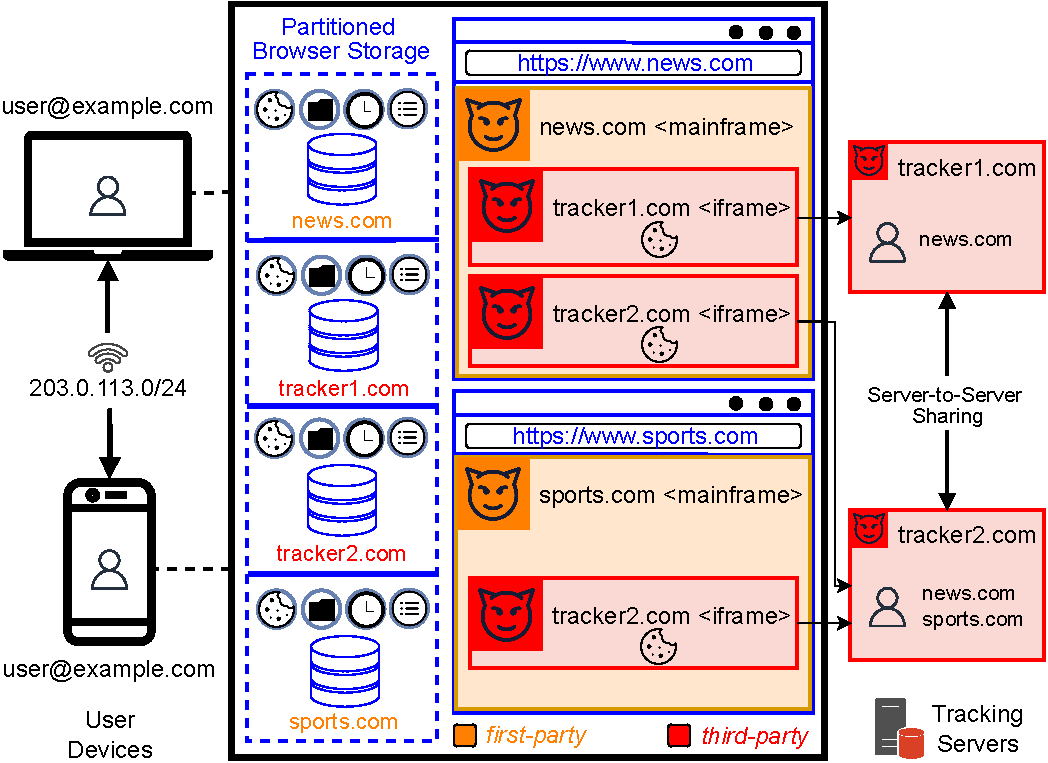
\includegraphics[width=0.99\linewidth]{figures/threat-model.pdf}
    \caption{Threat model of web tracking}
    \label{fig:threat-model}
    % \vspace{-6mm} % submission
    \vspace{-3mm} % arxiv
\end{figure}



%%
\noindent \textbf{Goals of an Adversary.} 
%
% The primary goal of an adversary is to identify and correlate user data across the web for purposes such as profiling, analytics, or ad targeting.
%
User data can be divided into two categories: (1) identifiers such as email or identifying information such as network, software, or hardware configurations, and (2) browsing activity comprising webpages visited and website interactions performed by the user. 
%
The tracker's goal can be distinguished into different scopes:
%
\noindent \textbf{\textit{Same-site}.} 
The tracker aims to monitor or recognize a returning user on the same first-party website across multiple visits or page loads. 
%
\textbf{\textit{Cross-site}.} 
%
Trackers embedded on multiple unrelated first-party websites often aim to uniquely identify and track a user across these sites in order to link different website activities to the same user.
%
\textbf{\textit{Cross-device}.} 
%
A tracker may also aim to identify the same user as they browse the internet using different devices or browsers. 
%
% For instance, \texttt{tracker1.com} embedded on \texttt{news.com} would like to know that the user \texttt{X} on a mobile phone is the same as user \texttt{Y} browsing the same website a little later from a desktop device.
%
In summary, the adversary's primary goal is to persistently and uniquely label the user or the user’s browser/device and to collect user data tied to that label, across navigations, sites, and over time, for purposes such as profiling, analytics, or ad targeting.
%
Besides, a secondary goal of the tracker may be to avoid detection or prevention---\ie{}, trackers aim to achieve their goal despite anti-tracking measures.


%%
\noindent \textbf{Capabilities of an Adversary.} 
%
% A tracker's capabilities are shaped by the web's architecture and browser's security model discussed in ~\autoref{sec:background}.
%
To achieve its goals, an adversary's capabilities can be explained in context of \textit{inclusion}, \textit{collection}, \textit{storage}, and \textit{sharing} of the user data, subject to the browser's context-origin restrictions discussed in ~\autoref{sec:background}.
%
The adversary is considered capable enough to track users either in presence of these browser-enforced policy restrictions or by circumventing them.
%
\textbf{\textit{Inclusion}.} 
%
A first-party tracker is assumed to directly monitor user activities within the mainframe context.
%
A third-party tracker could be embedded as an inline resource (\eg{}, image/script tag) within the mainframe context by the first-party assuming trust delegation, an iframe with a separate context under its origin (\ie{}, with its own DOM, state, and resources), or as a resource within a third-party iframe, isolated from the mainframe context. 
%
% By including an executable resource (\eg{}, script) on the webpage, tracker gains the ability to run code in the user’s browser, subject to script execution context requirements governed by browser's context model discussed in Section~\ref{sec:background}.
% %
% With an embedded non-executable resource (\eg{}, image), a tracker can still initiate resource loading requests to its server, sharing cookies along with the request.
% %
% We assume the tracker could use one or more inclusion methods described above depending on what the first-party allows.
%
\textbf{\textit{Collection}.}
%
A tracker aims to collect user data through available browser features by either executing JavaScript code or reading browser storage.
%
\textbf{\textit{Storage}.}
%
Trackers may read, write, or modify data in the user's browser using \texttt{localStorage}, \texttt{sessionStorage}, \texttt{indexedDB} and the cookie jar.
%
The stored data can be accessed by the tracker in subsequent visits to either the same site or a different site.
%
\textbf{\textit{Sharing}.}
%
Next, the adversary's goal is to share the collected user data with its own servers or a partner's tracking server.
%
For this, trackers can initiate network requests including the user data in one of four ways: (1)~as request URL query parameter, (2) request payload, (3)~request header, or (4) through HTTP cookies.
%
Approaches 1-3 require tracking scripts to explicitly include user data, whereas HTTP cookies associated with the tracker's domain are automatically included in all requests to the tracker's server. % (\eg{}, setting a custom request header for tracking).
%
% In case of 4, browsers automatically attach the previously set tracker's cookies with the requests sent to the tracker’s domain as a request header, even if that request originates in a first-party context. 
%%
We use this threat model to understand different web tracking mechanisms and their evolution over time.



%-------------------------------------------------------------------------------





%-------------------------------------------------------------------------------
%%
\section{Stateful Tracking}
\label{sec:stateful-tracking}
\vspace{-1mm}
%%
The most straightforward approach to tracking a user involves storing a unique identifier in their browser and retrieving it or modifying it as they browse different websites, which is a process known as ``stateful tracking''. 
%
Browsers provide a number of interfaces (\eg{}, cookies) that are designed to associate \textit{state} to the user's visit. 
%
Browsers also provide many interfaces that store information as a side effect of some other functionality provided to the website (\eg{}, E-Tags, HSTS upgrades), which trackers can sometimes abuse to encode a unique identifier~\cite{englehardtAutomatedDiscoveryPrivacy2018,ashkansoltaniFlashCookiesPrivacy2011,solomosTalesFaviconsCaches2021}.
%
% \noindent The capabilities of a tracker %depends on the restrictions 
% are governed by browsers security model defined in \autoref{sec:background}: (1) script execution privileges (2) context of inclusion (3) storage access policies.




%%
\subsection{Third-party Stateful Tracking}
\label{sec:tp-stateful}

\vspace{-1mm}
\subsubsection{Cookies} Cookies---first specified by Lou Montulli at Netscape in 1990s---allow maintaining a state when the browser communicates with a web server via HTTP, a stateless protocol~\cite{kristolHTTPCookiesStandards2001}. 
%
For example, a website can store a user’s authentication token in the browser via a cookie, which is then presented to the web server with each request that the user’s browser makes, allowing the website to verify the user’s authentication status. 
%
Browsers mediate which resources and domains are able to access specific cookies~\cite{beugin2024WebAlmanac2024,singhIncoherenciesWebBrowser2010,mdnSameoriginPolicySecurity2024}.

\begin{figure}[htbp]
    \vspace{-2mm}
    \centering
    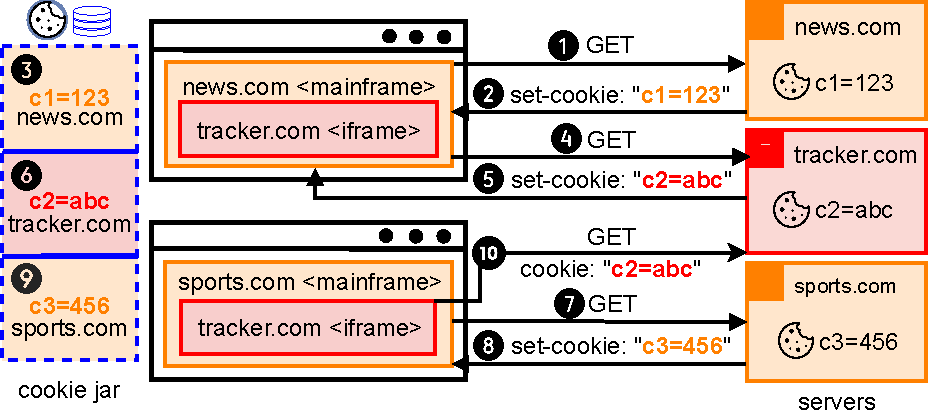
\includegraphics[width=1\linewidth]{figures/tracking-mechanisms-cookie.pdf}
    \vspace{-6mm}
    \caption{Cookie-based Tracking}
    \label{subfig:cookie-tracking}
    \vspace{-2mm}
\end{figure}

%%
First- or third-party domains on a webpage can set and receive cookies---either via \texttt{cookie} and \texttt{set-cookie} headers in network requests and responses respectively or via the \texttt{document.cookie} JavaScript method. 
%
In a first-party context, cookies allow a user to be re-identified to the website that they visit, while in a third-party context, it allows for cross-site tracking. 
%
For example, in \autoref{subfig:cookie-tracking}, \texttt{news.com} and \texttt{sports.com} both include iframes with ads from \texttt{tracker.com}. 
%
As a result, the user’s browser will send the same \texttt{tracker.com} cookie with requests to load the iframes on both pages. 
%
On \texttt{tracker.com} server's side, these two requests can be attributed to the same user and combined with additional information about the user-visited website. 
% (from the HTTP Referrer header or query parameters passed along when the request to load the iframe is made). 
%
Privacy concerns with third-party cookies were identified as early as their introduction~\cite{montulliHTTPStateManagement1997,kristolHTTPCookiesStandards2001} as public concern over web tracking elevated to the point where the FTC held a workshop on the topic in 1997~\cite{ftcWorkshopConsumerInformation1997}. 
% and the United States government banned and audited the use of cookies on government websites~\cite{SenatorRaisesPrivacy2001}. Nonetheless, this mechanism 
Nonetheless, cookies have been the dominant form of web tracking for many years. 

%%
\vspace{-1mm}
\subsubsection{Cookie Syncing}
%%
Third-parties included on a few websites, are only able to track users across that limited number of sites~\cite{roesnerDetectingDefendingThirdparty2012,lernerInternetJonesRaiders2016}. 
%
Moreover, under the SOP restriction, a third-party on a webpage cannot share its cookies with another third-party domain by directly initiating a request to it.
%
To overcome these constraints and exchange information collected about the user on different websites, third-party companies rely on cookie syncing or cookie matching~\cite{acarWebNeverForgets2014,englehardtOnlineTracking1millionsite2016,bashirTracingInformationFlows2016,papadopoulosCookieSynchronizationEverything2019,fouadMissedFilterLists2020,urbanMeasuringImpactGDPR2020}---first described by Olejnik et al.~\cite{olejnikSellingPrivacyAuction2014} and also named as ``referred tracking'' by Roesner et al.~\cite{roesnerDetectingDefendingThirdparty2012}. 

\begin{figure}[htbp]
    \vspace{-3mm}
    \centering
    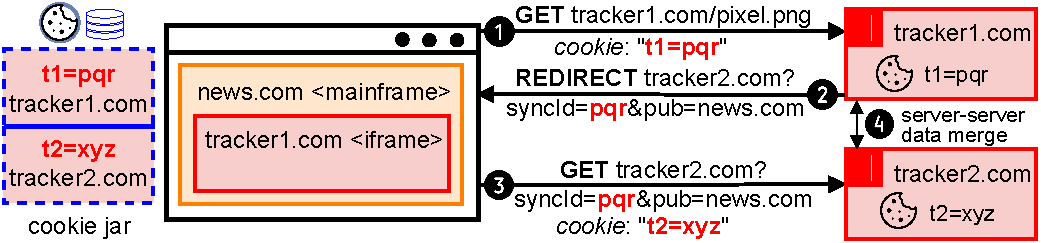
\includegraphics[width=1\linewidth]{figures/tracking-mechanisms-cookie-syncing.pdf}
    \caption{Cookie Syncing}
    \label{subfig:cookie-syncing}
    \vspace{-2mm}
\end{figure}

%%
This mechanism relies on synchronizing user identifiers known to two different third parties that are typically stored in third-party cookies and most commonly communicated via URL parameters. 
%
Following from the previous example, let’s suppose there are two trackers---\texttt{tracker1.com} and \texttt{tracker2.com}. 
%
If only \texttt{tracker1.com} is present on \texttt{news.com} as shown in \autoref{subfig:cookie-syncing}, it can share its user identifier stored in a third-party cookie by initiating a request to \texttt{tracker2.com} and adding it in the URL parameter. 
%
This would allow \texttt{tracker2.com} to know the identifier the user has for \texttt{tracker1.com}, match it with the user identifier of \texttt{tracker2.com}, and communicate server-to-server to further merge the information collected about this user by \texttt{tracker1.com} and \texttt{tracker2.com}. 


%%
\vspace{-2mm}
\subsubsection{Tracking Tags}
%%
Traditionally, tracking pixels (also called invisible pixels) used to be basic 1x1 image elements embedded on a webpage that pointed to some tracking endpoint.
%
When a user visits a webpage embedding a 1x1 pixel, user data is shared with the tracker, allowing user tracking on the same site as well as cross-site.
%
Image-based tracking pixels have been primarily used for analytics, ad (re)targeting, and conversion tracking. 
%
Researchers have conducted various large-scale measurements to study image-based tracking pixels \cite{Narayanan2017WebtapSpringer,englehardtOnlineTracking1millionsite2016,lernerInternetJonesRaiders2016, bekosHitchhikersGuideFacebook2023, agarwal2021under,vekaria2021differential}.

\begin{figure}[htbp]
    \vspace{-2mm}
    \centering
    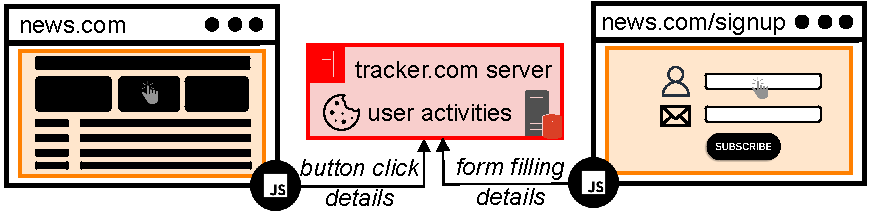
\includegraphics[width=1\linewidth]{figures/tracking-mechanisms-tracking-tags.pdf}
    \caption{Tracking Scripts}
    \label{subfig:tracking-scripts}
    \vspace{-2mm}
\end{figure}

%%
Over the years, tracking pixels have significantly advanced in their capabilities.
%
Modern tracking pixels, also referred to as tracking tags, rely on JavaScript to collect more fine-grained information in browsers. 
%
\autoref{subfig:tracking-scripts} represents a simple scenario where a tracking pixel from \texttt{tracker.com} is embedded on the homepage as well as on the \texttt{/signup} page of \texttt{news.com}, respectively collecting and sharing button clicks and form events with its own server, with the help of its tracking script.
%
Thus, tracking pixels have expanded in scope to support additional use cases, such as managing multiple pixels via a single tag, bot detection, and replaying of user sessions.




%%
\vspace{-1mm}
\subsection{First-party Stateful Tracking}
\label{sec:fp-stateful}
\vspace{-2mm}

%%
Since most browsers either block \cite{TrackingPreventionWebKit2020} or partition third-party access (by origin) to stateful APIs \cite{mdnThirdpartyCookiesPrivacy2024}, trackers aren’t able to store and retrieve identifiers \textit{across} sites. 
%
At best, storage partitioning allows tracking user activity on a single site.
%
To circumvent these protections, trackers adopt first-party based mechanisms described in this section.

%%
\vspace{-1mm}
\subsubsection{Cookies}
\label{subsubsec:stateful-tracking-cookies}
%%
When third-party tracking scripts are embedded into first-party execution contexts, the scripts execute with the same privileges as first-party scripts, allowing them to read and write JavaScript-accessible first-party storage as if they were a first-party script~\cite{bahramiCOOKIEGUARDCharacterizingIsolating2024}. 
%
First-party cookies often store unique user identifiers created with browser fingerprinting and those which are bounced through navigational tracking (see \autoref{sec:navigational-tracking}). 
%
Recent research \cite{munirCookieGraphUnderstandingDetecting2023,vekaria2024WebAlmanac2024} has shown that nearly 90\% of all websites use at least one tracking first party cookie, 96\% of which are in fact set by third-party scripts running in a first-party context.


%%
\vspace{-1mm}
\subsubsection{Cookie Syncing}
%%
One of the privacy issues with first-party cookies is syncing these identifiers with other third-parties. 
%
This sharing---first described by Fouad et al.~\cite{fouadMissedFilterLists2020}---allows third-parties to collude with each other and benefit from information gathered from users’ across different websites in a first-party context. 
%
In some cases, Google and Facebook set first-party cookies are shared with hundreds of other third-party domains~\cite{munirCookieGraphUnderstandingDetecting2023,bahramiCOOKIEGUARDCharacterizingIsolating2024}.
%
% In addition to syncing first-party cookies, trackers also combine personal information obtained from users across different websites to create extensive identity graphs of users as described in~\autoref{sec:id-providers} to track users in absence of third-party cookies.


%%
\vspace{-1mm}
\subsubsection{Tracking Tags}
%%
Blocking third-party cookies render tracking pixels embedded as image elements ineffective. 
%
However, modern tracking tags relying on JavaScript can still be used to track users in a first-party context~\cite{munirCookieGraphUnderstandingDetecting2023}. 
%
These tags are often included in the main frame context of a website by the developer, allowing pixel tracking companies to monitor different user activities using first-party execution privileges.


%%
\vspace{-1mm}
\subsubsection{Navigational Tracking}
\label{sec:navigational-tracking}
%%
A popular mechanism for sharing identifiers is via link decorations as depicted in \autoref{subfig:navigational-tracking}. 
%
Recent research has identified query parameters, resource paths, and URL fragments being used for sharing user data, such as first-party cookies and email addresses, on more than 70\% of websites~\cite{munirPURLSafeEffective2024}, in absence of third-party cookies or first-party partitioning. 
%
Besides link decorations, bounce tracking is another navigation-based mechanism that allows trackers to read/write their cookies across sites, rendering third-party cookie blocking ineffective~\cite{kellyBounceTrackingMitigations2022}. 


\begin{figure}[htbp]
    \vspace{-2mm}
    \centering
    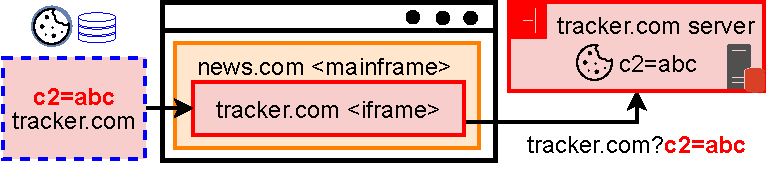
\includegraphics[width=1\linewidth]{figures/tracking-mechanisms-navigational-tracking.pdf}
    \caption{Navigational Tracking}
    \label{subfig:navigational-tracking}
    \vspace{-2mm}
\end{figure}

%%
At a high level, a tracker’s goal is to momentarily surface or visit its own domain in the browser’s \emph{first-party} context, because this lets it read and write identifiers that persist in first-party storage. 
%
\autoref{subfig:bounce-tracking} shows a typical \textbf{bounce-tracking} sequence:
%
\ding{182} A third-party script on \texttt{news.com} reads first-party identifier(s) stored under \texttt{news.com} and
%
\ding{183} includes them in the request to \texttt{tracker.com}.
%
\ding{184} Browser redirects to \texttt{tracker.com}—either by a user click or automatically (e.g., \texttt{window.location.href="...";} or a \texttt{<meta http-equiv="refresh">}).
%
\ding{185} Once loaded as a \emph{first party}, \texttt{tracker.com} reads the identifier from the URL or merges it with an existing cookie, rewriting the URL to its final destination (e.g., back to \texttt{news.com} or a different domain), embedding the consolidated identifier.
%
\ding{186} The browser navigates to \texttt{news.com}; the tracker’s script there extracts identifier from the decorated URL and 
%
\ding{187} stores it in \texttt{news.com}’s first-party storage, completing the cross-context linkage (if redirected to same first-party) or cross-site linkage (if redirected to a different domain).

\begin{comment}
% \begin{enumerate}[label=(\roman*)]
\begin{dingautolist}{182}
  \item A third-party script on \texttt{news.com} reads any first-party identifier already stored under \texttt{news.com}.
  \item Identifier is included in the request to \texttt{tracker.com}.
  \item Browser redirects—either by a user click or automatically (e.g., \texttt{window.location.href="...";} or a \texttt{<meta http-equiv="refresh">})—to \texttt{tracker.com}.
  \item Once loaded as a \emph{first party}, \texttt{tracker.com} reads the identifier from the URL or merges it with an existing cookie, rewriting the URL to its final destination (e.g., \texttt{sports.com}), embedding the consolidated identifier.
  \item Browser navigates on to \texttt{sports.com}; the tracker’s script there extracts identifier from the decorated URL and stores it in \texttt{sports.com}’s first-party storage, completing the cross-site linkage.
\end{dingautolist}
\end{comment}

\begin{figure}[htbp]
    \vspace{-2mm}
    \centering
    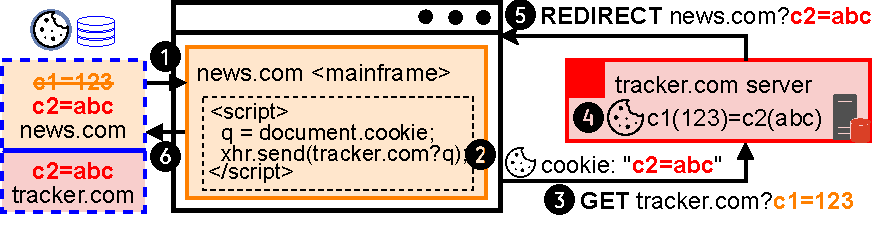
\includegraphics[width=1\linewidth]{figures/tracking-mechanisms-bounce-tracking.pdf}
    \caption{Bounce Tracking}
    \label{subfig:bounce-tracking}
    \vspace{-2mm}
\end{figure}

Bounce chains can involve two sites—\texttt{news.com} → \texttt{tracker.com} → \texttt{news.com}, or longer—allowing the tracker to propagate a stable user identifier across multiple seemingly unrelated websites despite third-party cookie restrictions.
%
% As a result of this process, a tracker is able to use the same identifier across websites. 
%
Due to potential usability disruptions and the implementation of defensive measures, bounce tracking is not widely pervasive
\cite{iqbalKhaleesiBreakerAdvertising2022}.
%
Measurements in 2020 found that 11.6\% of sites use one of the top 100 redirectors~\cite{koopInDepthEvaluationRedirect2020}, and in 2022 such identifiers were present in 8.1\% of the crawled navigations~\cite{randallMeasuringUIDSmuggling2022}.


%%
\subsection{Defenses Against Stateful Tracking}
\label{sec:stateful-defenses}
\vspace{-1mm}

Given the broad adoption of stateful tracking and its perceived intrusive nature, numerous tracking countermeasures have been proposed by the research community, some of which have either been adopted by browsers or are available to users through browser extensions.

%%
\vspace{-4mm}
\subsubsection{Third-party Stateful Tracking Protections}

%%
\paragraph{Clearing Cookies.}
Logically, a user could clear the cookies in their browser at the end of each session to protect themselves from being tracked. 
%
However, browser cookie clearing features do not typically clear \textit{all} stateful mechanisms provided to sites \cite{acarWebNeverForgets2014, englehardtOnlineTracking1millionsite2016}. 
%
For example, clearing cookies often does not remove identifiers stored in browser storage APIs \texttt{localStorage}~\cite{ayensonFlashCookiesPrivacy2011,roesnerDetectingDefendingThirdparty2012}, \texttt{IndexedDB}~\cite{acarFPDetectiveDustingWeb2013}, E-Tags~\cite{ayensonFlashCookiesPrivacy2011} and browser cache~\cite{sorensenZombiecookiesCaseStudies2013}
%
A malicious tracker can take advantage of this limitation by storing copies of their tracking identifiers in locations that aren’t cleared by the browser. 
%
Once a user clears their cookies, the tracker can use that hidden information to ``respawn'' or reconstruct the user’s identifier, creating a so-called ``supercookie'' or ``evercookie''~\cite{ayensonFlashCookiesPrivacy2011,soltaniFlashCookiesPrivacy2009,fouadMyCookiePhoenix2022}.
%
The most publicized example of supercookie was the Adobe's Flash browser plugin that provided no mechanism for browsers to clear its storage \cite{soltaniFlashCookiesPrivacy2009,solomosTalesFaviconsCaches2021}.
%
Any API that allows a tracker to persist state to the user’s device is a potential supercookie vector~\cite{aliNavigatingMurkyWaters2023}. 
%
Even just a single bit of storage can be abused if a tracker is able to string together multiple calls to an API, each encoding another bit from the identifier. 
%
Samy Kamkar first demonstrated how widespread this risk by encoding identifiers in APIs like HTTP Strict Transport Security (HSTS), Web Cache, \texttt{window.name}, and Web History~\cite{kamkarSamyKamkarEvercookie2010}. 
%
Variants of the same attack were also demonstrated later on other browser APIs~\cite{klink1334485TrackingUsing2017,goodinUnpatchedBrowserWeaknesses2015,evansPublicKeyPinning2015}. 
%
Ultimately supercookie risk was the prime motivation behind the network and storage partitioning efforts of Firefox, Chrome, and Safari~\cite{menkeStorageIsolationProject2020,privacycommunitygroupClientSideStoragePartitioning2022,mdnStatePartitioningPrivacy2024}. 
%
As of 2025, most browsers have blocked or partitioned third-party access to stateful APIs, preventing those APIs from being used to track users across websites.

%%
\vspace{-1mm}
\paragraph{Restrictions on Third-party Cookies.}
%
Browser vendors attempt to block most third-party cookies~\cite{mdnThirdpartyCookiesPrivacy2024} but leave some exceptions to support non-tracking use cases such as cookies that enable single sign-on (SSO), whose removal may lead to website breakage \cite{crouchImprovingPrivacyBreaking2018}. 
%
Privacy-focused browsers, such as Brave~\cite{braveBrowserThatPuts}, apply the most aggressive restrictions by blocking all third-party cookies by-default and allowing third-parties to share a partitioned ephemeral storage for the lifetime of the browsing session \cite{braveprivacyteamEphemeralThirdpartySite2021}. 
% (\ie{}, until the browser is closed or the last instance of first-party website (eTLD+1) closes)~\cite{braveprivacyteamEphemeralThirdpartySite2021}.
%
Among the mainstream browsers, Safari~\cite{appleSafari} and Firefox~\cite{mozillaGetFirefoxBrowser} have the most effective restrictions. 
%
Safari currently blocks all third-party cookies unless the domain (eTLD+1) has been visited by the user as a first-party or if the third-party explicitly requests to use the cookies through the Storage Access API~\cite{TrackingPreventionWebKit2020}. 
%
It further relies on an ML model to detect whether the domains with third-party access engage in tracking and restrict their cookies if the user has not interacted with the domain as a first-party in the last 30 days. 
%
Firefox blocks third-party cookies from known trackers (as determined by the Disconnect's tracking protection list~\cite{disconnectDisconnect}) and also partitions third-party cookies, such that each first-party and third-party origin combination has a separate cookie jar~\cite{mdnThirdpartyCookiesPrivacy2024}.
%
Initially, following in the footsteps of Safari and Firefox, Google Chrome~\cite{googleGoogleChromeFast} announced plans to block all third-party cookies~\cite{chromeBuildingMorePrivate2020}, which after several delays, it decided not to proceed with~\cite{chavezNewPathPrivacy2024}. 
%
Chrome currently offers various tools for developers to manage third-party cookies, including JavaScript APIs like the Storage Access API~\cite{mdnStorageAccessAPI2024} and cookie directives like the ``SameSite' attribute~\cite{mdnSetCookieHTTPMDN2024}. 
%
However, trackers may not adhere to or use these mechanisms. 
%
Moreover, they have migrated to alternative tracking techniques by circumventing existing protections.


\vspace{-1mm}
\paragraph{Blocking Trackers.}
%%
Filter lists are widely used by browsers (\eg{}, Brave) and browser extensions (\eg{}, uBlock Origin) to block third-party tracking requests.
%
However, filter list based ad or tracker blocking faces significant limitations: 
%
(1) manually curated lists are maintained by small community individuals and do not capture nuanced techniques. 
%
(2) as lists grow in size, they contain outdated or too narrow entries (\eg{} 90\% of EasyList rules are practically never triggered \cite{snyderWhoFiltersFilters2020}).
%
(3) being static, trackers keep evading them.
%
To overcome these challenges, researchers have focused on building ML-driven advertising or tracking request blockers ~\cite{iqbalAdGraphGraphBasedApproach2020, sibyWebGraphCapturingAdvertising2022, yangWTAGRAPHWebTracking2022, leAutoFRAutomatedFilter2023}.
%
AutoFR \cite{leAutoFRAutomatedFilter2023} proposes a fully automated framework for filter rule creation and evaluation.
%
While AdGraph \cite{iqbalAdGraphGraphBasedApproach2020}, WebGraph \cite{sibyWebGraphCapturingAdvertising2022}, and WTAGraph \cite{yangWTAGRAPHWebTracking2022} treat a webpage as a graph of HTML structure, network requests, and JavaScript behavior of a webpage to train a classifier for identifying and subsequently blocking advertising and tracking resources.
%
These approaches can generalize well to discover previously unknown trackers and adapt to evolving tracking behaviours. 
%
Brave implements an AdGraph-based ML solution (PageGraph) to detect and block trackers.
%
Beyond network requests, another popular anti-tracking method is to detect and block tracking scripts or JavaScript code at different granularities such as domain or path-based script blocking or function blocking within an otherwise benign script \cite{ikramSeamlessTrackingFreeWeb2016,alrizahErrorsMisunderstandingsAttacks2019,snyderWhoFiltersFilters2020,smithSugarCoatProgrammaticallyGenerating2021,chenDetectingFilterList2021,daoCNAMECloakingBasedTracking2021,leCVInspectorAutomatingDetection2021,amjadTrackerSiftUntanglingMixed2021,amjadBlockingJavaScriptBreaking2023,amjadBlockingTrackingJavaScript2024,ublockoriginUBlockOUBOScriptlets2025}.%
Adversarial trackers are incentivized to evade such blocking (\eg{} by changing script location or causing site breakage), posing challenges.


%%
\vspace{-4mm}
\subsubsection{Protections Against First-party Circumventions}

\paragraph{Restrictions on First-party Cookies.}
Unlike third-party cookies, first-party cookies cannot be as easily blocked completely because it would break critical website functionality such as maintaining login state. 
%
Therefore, they require more targeted countermeasures as listed below. 



%%
\vspace{-1mm}
\paragraph{Limiting the Lifetime of First-party Storage Written by Tracking Scripts.}
%
Safari’s Intelligent Tracking Protection (ITP) expires all first-party cookies or storage set by scripts post no user interaction for 7 days \cite{TrackingPreventionWebKit2020}. 
%
To mitigate workarounds that automatically overwrite cookies written by scripts with HTTP cookies, Safari detects third-party hosts cloaked under first-party subdomains using heuristics applied to the first-party host’s CNAME and IP address~\cite{TrackingPreventionWebKit2020}. 
%
Brave implements a limited version of this which caps the lifetime of cookies set by scripts to 7 days~\cite{bravePrivacyProtectionSecurity}. \\



%%
\vspace{-4mm}
\paragraph{Removing or Limiting the Persistence of Identifiers Passed in URL Parameters.}
%
Several browsers remove URL parameters known to be used by trackers. 
%
Firefox~\cite{mozillaQueryParameterStripping} implements removal in a non-default mode, while Brave~\cite{braveprivacyteamGrabBagQuery2020} and DuckDuckGo~\cite{duckduckgoDuckDuckGoWebTracking} ship it by default. 
%
When URL parameters are removed on navigation, tracking scripts embedded in the first-party context are prevented from accessing tracking IDs across sites. 
%
Safari takes a different approach: instead of removing tracking parameters, it limits the lifetime of script-accessible storage from 7 days to 24 hours when ITP detects link decoration~\cite{TrackingPreventionWebKit2020}.



%%
\vspace{-1mm}
\paragraph{Limiting First-party Storage Set During a Bounce.}
%
Bounce tracking not only circumvents third-party storage protections but also allows unrestricted access to tracker’s first-party storage. 
%
Browsers mitigate it by differentiating between a \textit{legitimate visit} to a site and a brief \textit{bounce} for tracking purposes. 
%
The fact that some authentication flows appear similar to bounce tracking complicates it~\cite{kellyBounceTrackingMitigations2022}. 
%
Brave and Firefox use blocklists to detect potential bounce trackers, whereas Safari and Chrome use heuristics based on site behavior as mitigations~\cite{snyderNavigationalTrackingMitigations2024}. 
%
Firefox, Chrome, and Safari delete all site storage for these domains unless there's an evidence of legitimate and recent user interaction with the site; the definition of \textit{legitimate} and \textit{recent} varies by browser~\cite{snyderNavigationalTrackingMitigations2024,TrackingPreventionWebKit2020}. 
%
While Brave provides suspected bounce trackers with access to ephemeral storage that’s cleared once all tabs opened from that tracker are closed, so long as the tracker doesn’t already have persistent storage set~\cite{braveprivacyteamUnlinkableBouncingMore2022}.

\vspace{-1mm}
\paragraph{Blocking First-party Cookies.}
Privacy-enhancing extensions support targeted deletion of known tracking cookies, including first-party cookies, through a filter list \cite{ublockResourcesLibrary,adguardrteamScriptletsWikiAboutscriptletsmd,schininaSourceBehavioralCookieremoverjs2024}.
%
While the filter lists face aforementioned challenges, they can also be automatically curated using a ML-based approach \cite{munirCookieGraphUnderstandingDetecting2023,bollingerAutomatingCookieConsent2022,schoniBlockCookiesNot2024a}.
%%
\vspace{-1mm}
\section{Stateless Tracking}
\label{sec:stateless-tracking}

%%
\vspace{-2mm}
\subsection{Browser Fingerprinting}
\label{sec:browser-fingerprinting}
\vspace{-2mm}

%%
Browser (or device) fingerprinting is a technique used to collect information on users’ browsers and devices. 
%
By using HTTP headers and calling specific JavaScript API endpoints, a website can collect a wide range of information on the browser and its configuration (\eg{} browser version, screen size, installed list of fonts, GPU model, timezone and preferred languages) to the underlying operating system and the hardware. 
%
Research has shown that the diversity of Internet-connected devices is so vast that the combination of collected attributes can be unique, leading to the identification of a specific device~\cite{eckersleyHowUniqueYour2010, laperdrixBeautyBeastDiverting2016,gomez-boixHidingCrowdAnalysis2018}. 
%
\autoref{fig:stateless-tracking} depicts how fingerprinting works.
%
Analysis of real-world fingerprints and entropy computations of all attributes have revealed that some attributes contribute a lot more to the uniqueness of users than others. 
%
Entropy~\cite{bacis2024assessing} measures the level of uncertainty or unpredictability in a dataset to understand how varied its distribution can be. 
%
For example, if a device's screen size can have 8 distinct values, its entropy is 3 bits.
%
Unlike techniques described in~\autoref{sec:stateful-tracking}, fingerprinting: 
%
1) does not rely on a stored state (\ie{} ID) in the browser to track a user as the fingerprint collection is performed in real-time to identify a device; 
%
2) is hard to detect and block; 
%
3) is also difficult to evade as users keep the same device for months or years, resulting in stable fingerprints over time.

\begin{figure}[htbp]
    \vspace{-2mm}
    \centering
    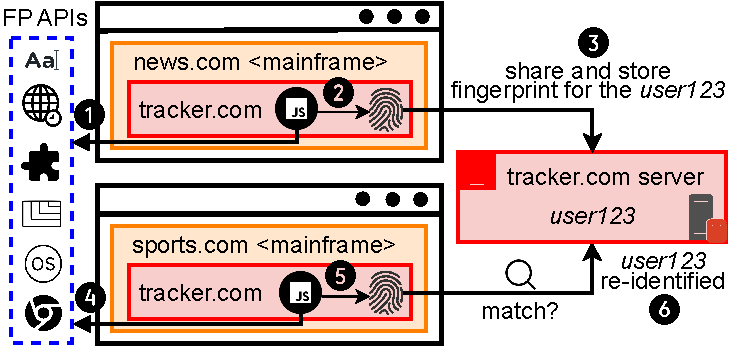
\includegraphics[width=0.8\linewidth]{figures/tracking-mechanisms-fingerprinting.pdf}
    \caption{Stateless Tracking via Browser Fingerprinting}
    \label{fig:stateless-tracking}
    \vspace{-2mm}
\end{figure}

%%
Since the first academic work on browser fingerprinting in 2009~\cite{mayerAnyPersonPamphleteer2009}, researchers have studied: its impact on privacy~\cite{eckersleyHowUniqueYour2010}, use with other tracking techniques~\cite{fouadMyCookiePhoenix2022}, its detection~\cite{iqbalFingerprintingFingerprintersLearning2021, boussahaFPtracerFinegrainedBrowser2024}, use in real world applications~\cite{aminazadWebRunner20492020, wuHimManyFaces2023}, abusable browser APIs~\cite{bahramiFPRadarLongitudinalMeasurement2022, suAutomaticDiscoveryEmerging2023, senolDoubleEdgedSword2024}, and user protections~\cite{vastelFpScannerPrivacyImplications2018}. 
%
In 2013, fingerprinting was observed on just $\sim$1\% of the top 10K websites~\cite{nikiforakisCookielessMonsterExploring2013} and $\sim$400 of the top 1 million websites~\cite{acarFPDetectiveDustingWeb2013}. 
%
Over the years, a variety of techniques have been used to measure browser fingerprinting~\cite{acarWebNeverForgets2014,englehardtOnlineTracking1millionsite2016,olejnikBatteryStatusNot2017,dasWebsSixthSense2018}, with two general trends being: its higher adoption by third-parties and its expansion to a diverse set of browser APIs over the years. 
%
By 2021, fingerprinting scripts were found to be present on 10\% of the top 100K websites, with more popular ones having a higher incidence (\ie{}, 30\% of the top 1,000)~\cite{iqbalFingerprintingFingerprintersLearning2021}.
%
Importantly, browser fingerprints are not always stable enough to track users over time: 80\% of browser instances change fingerprints in less than 10 days~\cite{vastelFPSTALKERTrackingBrowser2018}. 
%
Trackers not only link fingerprints as they evolve, but also combine and persist them with \textit{stateful} techniques, rendering effectiveness even in browsers that partition third-party access to stateful APIs (\autoref{sec:stateful-defenses}). 
%
A 2022 study showed a lower bound on this by detecting it on 1,150 of the top 30K sites~\cite{fouadMyCookiePhoenix2022}.
%
Other recent works indicate that fingerprinting risks differ across demographics~\cite{berkeHowUniqueWhose2025} and that limiting the information contained in fingerprints would not break the user experience~\cite{intumwayaseUARadarExploringImpact2023}.


%%
\vspace{-2mm}
\subsection{Types of Fingerprinting}
\label{sec:types-of-fingerprinting}
\vspace{-3mm}


%%
Besides browser fingerprinting techniques, researchers have demonstrated numerous side-channel approaches to track users.
%
One such approach is extension fingerprinting, aimed at inferring the presence of specific extensions in user's browser~\cite{karamiCarnusExploringPrivacy2020}. 
%
Early studies~\cite{sjostenDiscoveringBrowserExtensions2017, gulyasExtendNotExtend2018, karamiCarnusExploringPrivacy2020} demonstrated how extensions contain specific resources (\eg{}, images, scripts) that can be referenced by web pages, thereby revealing their presence in the user's browser. 
%
Researchers have also explored behavioral extension fingerprinting~\cite{starovXHOUNDQuantifyingFingerprintability2017, karamiCarnusExploringPrivacy2020, solomosDangersHumanTouch2022, solomosEscapingConfinesTime2022, laperdrixFingerprintingStyleDetecting2021, agarwalPeekingWindowFingerprinting2024}---where an extension can be implicitly inferred through executional side-effects---and corresponding mitigations~\cite{karamiUnleashSimulacrumShifting2022, sanchez-rolaExtensionBreakdownSecurity2017} such as randomizing WARs, IDs, or classes~\cite{trickelEveryoneDifferentClientside2019} and access control based extension loading~\cite{sjostenLatexGlovesProtecting2019}. 


%%
Apart from extension fingerprinting, prior works have explored various browser-supported JavaScript APIs for fingerprinting such as Canvas~\cite{moweryPixelPerfectFingerprinting2012}, WebGL~\cite{caoCrossBrowserFingerprintingOS2017}, Audio API~\cite{englehardtOnlineTracking1millionsite2016}, and the Battery Status API~\cite{olejnikLeakingBatteryPrivacy2016}. 
%
Sanchez-Rola et al. further demonstrated how JavaScript APIs can be used to construct a hardware fingerprint by analyzing the execution timing of instruction sequences~\cite{sanchez-rolaClockClockTimeBased2018}, while others have demonstrated browser-based fingerprinting techniques that target the device's CPU~\cite{trampertBrowserBasedCPUFingerprinting2022,matyuninTrackingPrivateBrowsing2018} or GPU~\cite{laorDRAWNAPARTDevice2022}. 
%
Recent research also demonstrates DRAM-based device fingerprinting capabilities from the vantage point of browsers~\cite{venugopalanFPRowhammerDRAMBasedDevice2024}.
%
Hardware-related fingerprints have also been extensively explored within the mobile ecosystem~\cite{bojinovMobileDeviceIdentification2014,dasTrackingMobileWeb2016,marcantoniLargescaleStudyRisks2019,hupperichRobustnessMobileDevice2015,deyAccelPrintImperfectionsAccelerometers2014,zhang2019sensorid}, due to the availability of additional sensors (\eg{}, gyroscope, magnetometer) which can exhibit unique hardware ``imperfections'' that occur during the manufacturing process. 
%
More broadly, any browser mechanism that extracts some form of data or affects client-side policies or behavior without storing a user-specific identifier, should be treated as a potential stateless tracking vector and analyzed accordingly~\cite{aliNavigatingMurkyWaters2023}. 
%
Generally, side-channel attacks are challenging to detect and could be equally difficult to mitigate.


%%
\vspace{-1mm}
\subsection{Need for Fingerprinting}
\label{sec:need-for-fingerprinting}
\vspace{-2mm}

%%
Constructively, fingerprinting can be thought of as a form of intrusion detection. 
%
Web applications can learn about the browsing environment of their first-party users and associate it with specific user identities~\cite{LinPhishSheepsClothing2022}. 
%
For example, a website can learn that the user Alice is using a smartphone with specific dimensions or a desktop browser with a specific kind of GPU. 
%
If Alice's credentials are ever stolen and an attacker attempts to login to that service, the service can extract the attacker's fingerprint, observe a major difference against Alice's fingerprints from prior sessions, and request additional authentication data from the attacker (such as a one-time password).
%
The same techniques can be constructively used to differentiate real users from malicious bots, as well as attackers engaging in ad fraud.


%%
Destructively, the same techniques that can identify user-impersonating attackers and bots, can be turned against users who wish to keep their identity anonymous. 
%
Using fingerprinting, a web application may be able to determine that a certain anonymous user is in fact eponymous, since their browser fingerprint matches that of a known user on the same platform. 
%
This undesired re-identification occurs despite user's attempt to hide by deleting their cookies or using the browser's private mode. 
%
In a cross-site context, fingerprinting can be abused to link unrelated website visits together, even when third-party cookies are disabled.


%%
\vspace{-1mm}
\subsection{Defenses Against Stateless Tracking}
\label{sec:stateless-defenses}
\vspace{-2mm}

%%
Browser vendors consider fingerprinting as a form of covert tracking that’s harmful to the web~\cite{nottinghamUnsanctionedWebTracking2015}. 
%
All major browsers have deployed some mitigations against fingerprinting and the W3C encourages specification authors to consider how their APIs contribute to the fingerprinting surface of the browser~\cite{dotyMitigatingBrowserFingerprinting2019}. 
%
Despite this, major browsers continue to expose a significant amount of information that can be used to fingerprint users.
%
There is no optimal strategy against fingerprinting as it often comes at the cost of user's utility. 
%
There is rather a disagreement between vendors on the feasibility of completely mitigating fingerprinting and the value of deploying incremental improvements without a clear path to complete mitigation~\cite{snyderBraveFingerprintingPrivacy2019, rescorlaTechnicalCommentsPrivacy2021}. 
%
% As such, fingerprinting mitigations vary greatly across browsers.

%%
The most common approach to mitigating fingerprinting is the normalization of device information exposed by browsers to reduce the utility of fingerprints. 
%
Browsers such as Tor make all users appear to have the same fingerprint, thereby making it hard to differentiate between them~\cite{perryDesignImplementationTor2013}. 
%
Whereas others introduce randomness so that a single user's fingerprint keeps changing from page load to page load, complicating user tracking. 
%
These latter countermeasures are easier to deploy across user populations and hence more popular than the ones which aim to make all environments appear identical.
%
Browser vendors have reduced identifying information exposed by APIs already shipped to the web, have removed web APIs known to be abused for fingerprinting, and have declined to implement new APIs that expose additional fingerprinting surfaces. 
%%
Examples include: freezing the minor browser version from the User-Agent string~\cite{weissIntentDeprecateFreeze2020}, unshipping the Battery Status API due to being fingerprintable~\cite{olejnikBatteryStatusNot2017}, and WebKit and Firefox’s refusal to implement the Network Information API, in part, due to fingerprinting concerns~\cite{TrackingPreventionWebKit2020, thomsonNetworkInformationAPI2018}.


%
Web API normalization sometimes breaks websites that expect to have access to device information. 
%
% For example, Mozilla rolled back their effort to freeze the Android OS version in Firefox for Android’s User-Agent string due to breakage on a major authentication provider~\cite{peterson1865766FreezeAndroid2024}. 
%
For web APIs that can’t be normalized, browsers have added site-specific randomized noise to the outputs of those APIs, for example, noise added to the rasterized outputs of the 2D Canvas, to WebGL renderings, and \texttt{AudioBuffer} samples from the WebAudio API. 
%
Randomization was first deployed by Brave under the name ``farbling’’~\cite{braveprivacyteamFingerprintingDefenses202020}, and was later adopted by Firefox~\cite{huang1816056FprandomizationMeta2023} and Safari~\cite{wilanderPrivateBrowsing202024}. Crucially, alternative fingerprinting techniques can still be employed~\cite{linFashionFauxPas2023}.


%%
Besides changes to individual API outputs, browsers have also explored approaches grounded in policy to discourage fingerprinting. 
%
Mozilla released an anti-tracking policy which forbids browser fingerprinting~\cite{mozillaSecurityTrackingPolicy2019} and subsequently blocked scripts from loading in Firefox when they were detected to include browser fingerprinting code~\cite{englehardtFirefox72Blocks2020}. 
%
Google Chrome engineers proposed a \textit{Privacy Budget} on websites where websites would be allowed to access fingerprintable device information up to a browser-defined budget~\cite{lasseyMikewestPrivacybudget2019}.
%
Once that budget is exceeded, the browser would limit the further exposure of identifying information. 
%
This approach was met with skepticism due to a likelihood of website breakage and risk of exposing additional tracking surface~\cite{snyderBraveFingerprintingPrivacy2019, rescorlaTechnicalCommentsPrivacy2021}, resulting in its discontinuation~\cite{leflerWhatHappenedPrivacy2024}. 
%
Thus, a lack of unified effort in the past decade to tackle fingerprinting suggests that, as of now, there is no desire in the tech community to remove it entirely. 
%%
\vspace{-2mm}
\section{Cross-device Tracking}
\label{sec:cross-device}
\vspace{-4mm}

\paragraph{Types of Cross-device Tracking.} Cross-device tracking can be \textit{deterministic} or \textit{probabilistic}~\cite{kimProbabilisticVisitorStitching2017,cottaOffPolicyEvaluationProbabilistic2019,brookmanCrossDeviceTrackingMeasurement2017}. Traditionally, user’s account information such as username or email addresses have been used to link or associate browsing activity across devices. When these deterministic identifiers fail, for example, if the user is logged out, probabilistic signals are used such as (a) IP addresses shared by multiple devices belonging to the same user~\cite{diaz-moralesCrossDeviceTrackingMatching2015}, (b) URL browsing patterns since people tend to visit the same websites and apps across devices~\cite{phanCrossDeviceMatching2017}, (c) OS and hardware characteristics~\cite{caoCrossBrowserFingerprintingOS2017}, or (d) typing behavior~\cite{yuanCrossdeviceTrackingIdentification2018}. These features are combined by trackers into \textit{cross-device graphs}~\cite{zimmeckPrivacyAnalysisCrossdevice2017,wangGraphTrackGraphbasedCrossDevice2022}.

\para{Limitations.} However, probabilistic techniques do not always provide a reliable identifier (\eg{} ISPs dynamically rotate and share public IP addresses across several households). As a result, trackers employ proprietary algorithms to eliminate noise, such as ignoring commercial, private, and proxied IP ranges from cross-device graph computations, or setting fine temporal thresholds for observed identifiers to be considered originating from the same user.

\para{Regulation.} To inform the ad industry of the privacy-invasive nature of cross-device tracking, the FTC held a cross-device tracking workshop in 2015~\cite{ftcCrossDeviceTracking2015}. It also issued warning letters to developers integrating Silverpush, an ad network performing cross-device tracking via inaudible ultrasound signals~\cite{ftcFTCIssuesWarning2016}. Various subsequent studies~\cite{mavroudisPrivacySecurityUltrasound2017,arpPrivacyThreatsUltrasonic2017,matyuninTrackingPrivateBrowsing2018} highlighted the invasiveness of this technique. 

\para{Defenses Against Cross-device Tracking.} Deterministic cross-device tracking protections are inherently limited by user's account login from different devices. On the other hand, probabilistic cross-device protections are, principally, the same as against traditional tracking, \eg{}, limiting the disclosure of user data that could be used to correlate users. 
On mobile devices, techniques have been introduced to intercept, inspect, and block outgoing packets from apps~\cite{shubaNoMoAdsEffectiveEfficient2018}. With respect to the use of inaudible ultrasound signals, efforts have pushed for the standardization of beacons and OS-level APIs to better control access to the functionality and selectively suppress certain frequencies~\cite{mavroudisPrivacySecurityUltrasound2017}.


%%
\vspace{-2mm}
\section{Measurement Methodologies}
\label{sec:measurement-methodologies}

%%
\vspace{-3mm}
\subsection{Crawling Measurements}
\label{sec:crawling}
\vspace{-2mm}

Web crawling with instrumented browsers is the most common approach to measure online tracking.
Browser instrumentation can take two forms: \textit{out-of-band} or \textit{in-band}. Out-of-band, or deep instrumentation, modifies directly the browser or JavaScript engine. In contrast, in-band leverages instrumentation hooks, like prototype patching, at the JavaScript level to overwrite functionality of interest.

\para{User Agent.} Most measurements require a browser supporting modern web features.
Simplified user agents which do not execute JavaScript or have incomplete support for web APIs can be appropriate for targeted measurements~\cite{apache-nutch}. 

\para{Automation Frameworks with Instrumentation Hooks.} To drive full consumer browsers, researchers rely on automation tooling built for website and browser testing: \eg{}, Chrome DevTools Protocol (CDP) for Blink-based browsers and Marionette for Gecko-based browsers. These internal interfaces are used by cross-browser automation libraries like Selenium or Puppeteer~\cite{
cross-browser-testing-1-2020,cross-browser-testing-2-2021,puppeteer-support-firefox-2024}.
Many researchers make direct use of these libraries, while several projects which bundle full browser automation with additional instrumentation and measurement tooling also exist~\cite{englehardtOnlineTracking1millionsite2016,openwpm4StudiesUsing,mayerFourthpartyFourthpartyFourthParty2011,duckduckgoDuckduckgoTrackerradarcollectorModular2020,libertWebXrayPrivacySearch2024}.

\para{Deep Instrumentation.} Many attempts have been made in leveraging deep instrumentation for security-related web measurements~\cite{neasbittWebCapsuleLightweightForensic2015,liJSgraphEnablingReconstruction2018, acarFPDetectiveDustingWeb2013, IncontextStoreIncontext1998, chenMystiqueUncoveringInformation2018}. The fundamental problem is that the browser evolves rapidly, rendering research prototypes obsolete quickly, as maintaining the patches is difficult or impossible~\cite{chenMystiqueUncoveringInformation2018}.  
Two major efforts try to overcome this limitation: VisibleV8~\cite{jueckstockVisibleV8InbrowserMonitoring2019} and PageGraph~\cite{bravePageGraph,braveBravePagegraphcrawl2025}.
%
PageGraph is maintained directly by the Brave Browser team, making it the only deep instrumentation framework that has browser support. 
%
VisibleV8 is designed so that its patches are minimal (67 lines of code for the actual JavaScript monitoring) and has been successful in providing builds from Chromium 63 to 137 (version at submission time) with minimal effort~\cite{wspratncsuWsprncsuVisiblev82025, jueckstockVisibleV8InbrowserMonitoring2019}. A major benefit is that deep instrumentation is agnostic to what needs to be monitored: \textit{all} web APIs can be hooked, even when not knowing the responsible APIs beforehand~\cite{suAutomaticDiscoveryEmerging2023}.

\para{Stealthiness.}
A significant threat to the validity of active web measurements is the ability of websites to detect crawlers and instrumented browsers. Upon detection, websites may block crawlers or alter their behavior (a practice known as \textit{cloaking})~\cite{invernizzi2016cloak}. Automation frameworks often inject detectable artifacts in the JavaScript context or alter the user-agent string. Researchers may need to deploy further evasion techniques~\cite{berstendPuppeteerextrapluginstealth2023} to avoid differential treatment.

\para{Site lists.} Top lists of popular websites are published by several sources based on different methodologies: Alexa Top Million~\cite{amazonAlexa} (now deprecated), Cisco Umbrella Popularity List~\cite{ciscoCiscoUmbrellaPopularity}, Majestic Million~\cite{majesticMajesticMillion}, Tranco~\cite{lepochatTrancoResearchOrientedTop2019}, Google CrUX~\cite{googleChromeUXReport2017}, or Cloudflare Radar~\cite{cloudflareCloudflareRadar2025}. 
%
Their use as a proxy to study websites and real users' behaviors has raised some skepticism in the past as these lists can be unstable, inconsistent, and prone to manipulation. Moreover, the choice of top list can sometimes impact research findings~\cite{lepochatTrancoResearchOrientedTop2019,ruthTopplingTopLists2022}.

\para{Existing Crawl Datasets.}
Another strategy is to leverage existing web crawl datasets. Nonprofit organizations and community-driven projects such as the Internet Archive~\cite{InternetArchiveDigital}, Common Crawl~\cite{commoncrawlCommonCrawlOpen}, and the HTTP Archive~\cite{httparchiveHTTPArchive} routinely crawl websites and publish their data openly.

\para{Limitations.} Representativeness and generalizability issues arise due to 
bot detection measures~\cite{krumnowHowGullibleAre2022},
measurement vantage points~\cite{samarasingheGlobalPerspectiveWeb2019},
device form factors~\cite{yangComparativeMeasurementStudy2020,casselOmniCrawlComprehensiveMeasurement2022}
and potential differences in results obtained from crawls versus real browsing by humans~\cite{zeberRepresentativenessAutomatedWeb2020}. Directly related, studies are often very difficult to reproduce and replicate as differences in methodologies and experimental setups are not always fully documented by researchers~\cite{demirReproducibilityReplicabilityWeb2022,hantkeWebExecutionBundles2025}.


%%
\vspace{-2mm}
\subsection{User Studies}
\label{sec:user-studies}
\vspace{-3mm}
%%

In practice, user studies can take multiple forms; they can be conducted through \textit{usability surveys or interviews}, or be based on data collected from real users through \textit{field measurements, crowdsourcing, or direct collection} through a browser extension or application. As an example, the National Internet Observatory~\cite{steningUnprecedentedDataCollection2022,nioNationalInternetObservatory,callahanCanWeBetter2021,fealIntroductionNationalInternet2024}, a nascent effort, invites US residents to volunteer data about their online behaviors and allows privacy-preserving access to researchers for scientific studies.
%
With these techniques, researchers have mostly investigated participants’ comprehension, perception, and interaction with respect to cookie  dialogs~\cite{birrellSoKTechnicalImplementation2024,machuletzMultiplePurposesMultiple2020,bermejofernandezThisWebsiteUses2021,habibOkayWhateverEvaluation2022,singhWhatCookieConsent2022,bielovaSurveyAcademicStudies2022,Bielova2024-zr}. They typically study and compare different consent dialog designs, finding that many current designs effectively nudge participants towards more privacy-preserving options~\cite{machuletzMultiplePurposesMultiple2020,bermejofernandezThisWebsiteUses2021}. These studies also recommend that consent choices be \textit{reject by default} and that users should be able to easily revisit choices they have made~\cite{habibOkayWhateverEvaluation2022,Kanc-etal-25-PETs}.


\begin{figure*}[t]
    % \vspace{-6mm} % submission
    \centering
    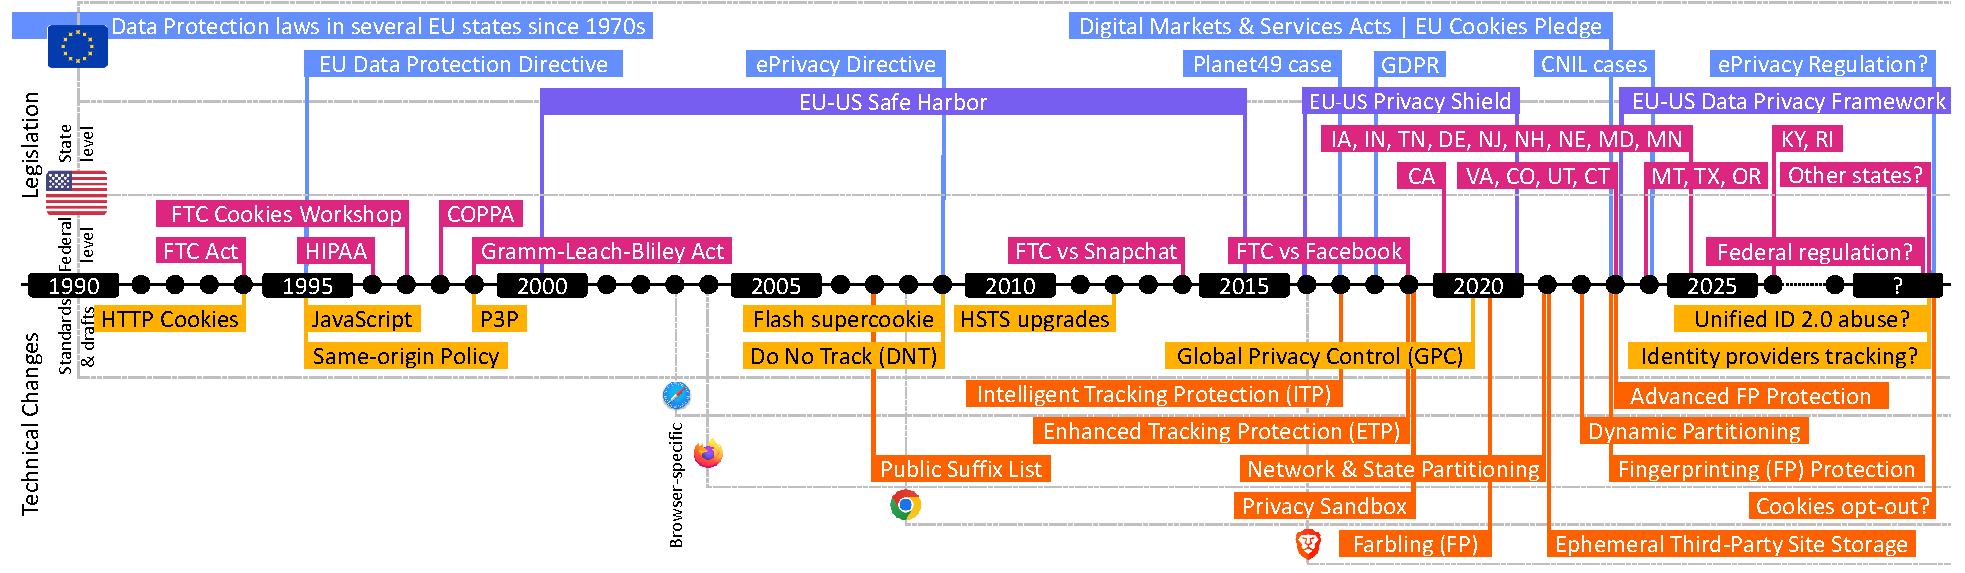
\includegraphics[width=\textwidth]{figures/timeline.pdf}
    \caption{Timeline of major technical and browser-specific changes with regulation overview in the EU and US.}
    \label{fig:timeline}
    \vspace{-4mm}
\end{figure*}
%-------------------------------------------------------------------------------



%-------------------------------------------------------------------------------
%%
\vspace{-2mm}
\section{Privacy Regulations}
\label{sec:regulations}

\vspace{-3mm}
\para{Regulatory Actions in the US.}
\label{sec:us-regulations}
% \vspace{-2mm}
%%
In the US, states enact their own privacy legislation and only a few narrow privacy laws exist at the federal level, notably for children’s personal data (COPPA)~\cite{ChildrensOnlinePrivacy2013}, protected health (HIPAA)~\cite{rightsocrHIPAAPrivacyRule2008}, and personal financial (Gramm–Leach–Bliley Act)~\cite{GrammLeachBlileyAct2013} information. Thus, apart from mandatory provisions, the notice and choice principle---generally implemented via privacy policies---governs what a recipient of personal information can do with it~\cite{zimmeckInformationPrivacyLaw2013}. 
%
Research has surveyed this principle~\cite{schaubDesignSpaceEffective2015} and has shown that it suffers from a lack of regulatory enforcement~\cite{cranorNecessaryNotSufficient2012}, vagueness and ambiguity of notices~\cite{reidenbergAmbiguityPrivacyPolicies2016}, unusable choice implementations~\cite{habibItsScavengerHunt2020}, and nudging and inconvenience factors~\cite{oconnorUnclearInconspicuousRight2021}.

Under its jurisdiction, the FTC can consider privacy policies that misrepresent a business's data handling practices as unfair or deceptive, affecting commerce per 15 U.S.C. §45(a)(1)~\cite{unitedstates:congress:houseofrepresentatives:officeofthelawrevisioncounselUnfairMethodsCompetition2023}, and has done so in the past~\cite{ftcSnapchatSettlesFTC2014,FTCImposes52019}. With such enforcement actions over the last few decades, the FTC has effectively created a body of common law of privacy~\cite{soloveFTCNewCommon2013}.  
%
Similarly, state attorneys general also increased their regulatory activity based on new state privacy laws: California passed the CCPA in 2020 and CPRA in 2023, soon followed by other states as depicted in~\autoref{fig:timeline}.
%
The systematization and enforcement of privacy laws in the US (and elsewhere) is advancing, though recent changes to the CCPA via the CPRA may negatively impact the usability, scope, and visibility of the right to opt-out of sale~\cite{charatanTwoStepsForward2024}.

%%
\para{Regulatory Actions in the EU.}
\label{sec:eu-regulations}
% \vspace{-2mm}
%%
Several EU states established the first data protection laws in late 1970s~\cite{LoiNdeg78171978,GermanDP-1977,NorwayDP-1978}, followed by the EU Data Protection Directive in 1995~\cite{Directive199546EC}, and the GDPR applicable to all EU member states in 2018~\cite{Regulation2016679}.  
%
Personal data transfers from the EU to the US are currently regulated by the EU–US Data Privacy Framework~\cite{EU-US-DP-2023} that replaced prior invalidated frameworks~\cite{PrivacyShield-2016,Schrems-II,SafeHarbor-2000,Schrems-I}.
%
The ePrivacy Directive (2002, amended in 2009) requires in its Article 5(3) a valid user’s consent before \textit{``storing of information, or the gaining of access to information already stored, in the terminal equipment’’}~\cite{Directive2002582002,Directive20091362009}. The GDPR re-defined this notion by setting higher-level legal requirements~\cite{santosAreCookieBanners2020}. As efforts to update the ePrivacy Directive into a Regulation have not reached a consensus so far~\cite{europeancommissionProposalEPrivacyRegulation2024}, EU regulators continuously update their national laws and compliance guidelines to further interpret and implement the ePrivacy Directive~\cite{Bielova2024-zr}.

Therefore, Article 5(3) of the ePrivacy Directive was interpreted in different ways to (a) require consent before cookies are set, read, or sent to third-parties, (b) establish that consent is not required for all tracking technologies if their use is \textit{``strictly necessary’’} (\eg{}, for load balancing) or needed for \textit{``enabling the communication’’}, and (c) cover various types of devices (such as mobile and IoT) and technologies (tracking pixels, link decoration)~\cite{Guidelines22023}. 
%
EU regulators have also been actively investigating tracking technologies, consent, and malpractices. In the Planet49 case, the highest court in the EU (CJEU) established legal precedent by declaring pre-ticked boxes in consent design interfaces illegal~\cite{CJEUC67317}. Similarly, the French Data Protection Authority found that consent banners must offer a reject option on the first layer~\cite{ClosureInjunctionIssued2023,CNILFranceSAN2021024}, and companies were fined for setting cookies prior to consent~\cite{CNILFranceSAN2020012,DeliberationSAN20200127} (for more decisions, see GDPRhub~\cite{GDPRhub}).

In recent years, the EU Commission %’s Cookie Pledge 
tried to establish simpler consent rules~\cite{europeancommissionCookiePledgeEuropean2023}, and EU laws, such as the Digital Markets Act~\cite{RegulationEU20222022} and Digital Services Act~\cite{RegulationEU20222022a} have set up additional rules on valid consent for major companies (defined as \textit{``gatekeepers’’}) and for dark patterns and advertising on online platforms, respectively.

%%
% \vspace{-1mm} % submission
\para{Policy-oriented Solutions.}
\label{sec:policy-solutions}
% \vspace{-2mm}
%%
Several attempts were made at implementing opt out and consent signals for users to communicate their privacy preferences to services. However, the adoption and enforcement of such signals by both senders and recipients is an unresolved coordination problem~\cite{hilsPrivacyPreferenceSignals2021}.

\noindent \textbf{\textit{Platform for Privacy Preferences Project (P3P)}}~\cite{reaglePlatformPrivacyPreferences1999,cranorPlatformPrivacyPreferences2002,cranorPlatformPrivacyPreferences2006} enabled websites to communicate their privacy practices to users in a standardized and fine-grained format. Nonetheless, its utility was limited by the low number of sites that were adopting it~\cite{cranorUseP3PUser2002} and those implementing it correctly and transparently~\cite{cranorAnalysisP3PDeployment2003, leonTokenAttemptMisrepresentation2010}.

\noindent \textbf{\textit{Do Not Track (DNT)}}~\cite{fieldingTrackingPreferenceExpression2019}, developed in 2009 as a binary opt out signal, also saw its adoption to remain low. Indeed, COPPA, which influenced the design of DNT, only requires online services to say whether or not they respect it~\cite{CaliforniaCodeBPC2003}.

\noindent \textbf{\textit{Global Privacy Control (GPC)}}~\cite{zimmeckGlobalPrivacyControl2024} can be viewed as a successor to DNT. While people find GPC useful and usable, adoption is slow~\cite{zimmeckUsabilityEnforceabilityGlobal2023,zimmeckGeneralizableActivePrivacy2024}, despite GPC compliance being required in California (2021)~\cite{archive-attorneygeneralbecerra[@agbecerra]CCPARequiresBusinesses2021,bontaAttorneyGeneralBonta2022} and Colorado (2024)~\cite{coloradodepartmentoflawUniversalOptOutShortlist2024}. Whether GPC can be applicable in the EU within ePrivacy and GDPR context, is still an open discussion~\cite{berjonGPCGDPR2021}.

Policy-oriented protocols and frameworks remain in early stages, as evidenced by the Data Rights Protocol~\cite{consumerreportsDataRightsProtocol2024} and industry consent frameworks~\cite{iabtechlabGlobalPrivacyPlatform2024}.

%-------------------------------------------------------------------------------




%-------------------------------------------------------------------------------
%%
\vspace{-1mm}
\section{Discussion \& Future Outlook}
\label{sec:future-outlook}
\vspace{-1mm}

\subsection{Stateful Tracking}
\vspace{-4mm}
\paragraph{Shift to First-party Cookies \& Cookie Partitioning.}
Nearly half of the top most visited websites already use first-party tracking cookies. We expect this trend to continue with further adoption of third-party tracking restrictions, content-blocking tools, and partitioning.
%
Cookie partitioning is a method by which cookies are siloed or ``partitioned’’ according to the context in which they are set, effectively restricting browser-based storage to remain strictly tied to each visited site, making it more difficult to link user identities and behaviors across different sites.
%
Nevertheless, partitioning is best viewed as one step in a need for a broader set of privacy measures: trackers can still use fingerprinting and first-party scripts embedded on individual domains.

%%
\begin{opbox}
In a world without cookies, what alternative forms of user tracking might emerge that could increase privacy risks, and how might these risks manifest---for example, in light of Chrome’s recent decision not to deprecate third-party cookies anymore?
\end{opbox}
\vspace{-3mm}


\paragraph{More Reliance on First-party Data \& Identity Graphs.}
\label{sec:id-providers}
As restrictions are being put in place on third-party cookies, websites now lean on a handful of major \emph{identity providers} (\eg{}, Google\,/\,YouTube, Facebook\,/\,Meta, Apple) who, through their position of gatekeepers, can authenticate users while quietly attaching persistent, service-specific identifiers. 
%
Many platforms further fuse this stream with in-house ``first-party’’ and offline data such as loyalty-card and point-of-sale data, constructing proprietary \emph{identity graphs} that map a single user (or household) to multiple browsers, apps, and physical transactions.
%
While these integrations help publishers measure conversions and personalize content under tighter browser policies, they also concentrate behavioral insight in a few dominant actors and erode users’ ability to maintain separate or pseudonymous personas, raising fresh antitrust and privacy challenges~\cite{TargetedAdvertisingAutorite2025,khanAmazonsAntitrustParadox2017,munirGooglesChromeAntitrust2024}.

\begin{opbox}
How can we detect or infer opaque server-side data flows, reveal what information is shared server-side, and quantify its privacy risks?
\end{opbox}
\vspace{-3mm}

\paragraph{Tracking Tags.}
%%
A tag from a given pixel tracking company can be configured in many ways depending on the distinct user behaviors websites want to track. As a result, detecting the mere presence of tracking pixels is not enough, and it is crucial to detect all JavaScript-based tracking tags embedded on a website, and study their tracking configurations to truly understand the tracking capabilities of such tags.
%%
\begin{opbox}
How are tracking tags configured differently, and what impact do these differences have on tracking behavior?
\end{opbox}
\vspace{-3mm}


\paragraph{Session Replays.}
Session replay (or recording) scripts capture detailed user interactions such as keystrokes, mouse, and scrolling movements, along with the full content of the visited pages.
%
This allows publishers to record and playback visits as if they are ``looking over [visitors’] shoulders’’, for purposes including marketing, analytics, and troubleshooting~\cite{AdvancedUsageInspectlet}.
%
However, these scripts can also capture sensitive personal data filled out by visitors~\cite{acarNoBoundariesData2020,senolLeakyFormsStudy2022,yuGotSickTracked2022}, while redaction measures offered by session replay vendors are often fragile and limited in effectiveness~\cite{englehardtNoBoundariesCredentials2018,acarNoBoundariesData2020}.

\vspace{-2mm}
\subsection{Stateless Tracking}
\vspace{-4mm}

\paragraph{Paywalls to Force Users to Remain Recognizable.}
To avoid limitations imposed by ad blockers~\cite{koreacopyrightcommissionNumberAdblockUsers2024}, some websites use paywalls or registration walls that require user authentication (and often payment information) before granting content access.
%
This tactic may reduce users' motivation to block cookies or browse privately, it also requires users to remain ``recognizable’’, giving website operators a reliable identifier that persists across sessions and is more robust than third-party cookies.
%
While paywalls may support legitimate revenue models---especially for publishers facing declining ad revenues---they also create an environment where anonymity is traded for access.
%
Consequently, if paywalls become more pervasive, it may be hard for privacy-conscious users to avoid sharing their personal data online.

%%
\begin{opbox}
How do publishers leverage paywalls to build and enrich first-party profiles, and how do they associate authenticated user identities with online behaviors (\eg{}, shopping) to enable targeted advertising within their own networks?
\end{opbox}
\vspace{-3mm}


\paragraph{Server to Server Data Sharing}
%
To circumvent ad blocking techniques, trackers have been shifting part of their tracking logic from client to server-side~\cite{fisherImprovePerformanceSecurity2020}.
%
Companies like Google, Meta, Amazon, or TikTok have deployed so-called \textit{conversion APIs} that, along with \textit{data clean rooms}, allow marketers to perform joint analysis of their own data with the one held inside these walled gardens in a privacy-preserving way.
%
But, \textit{server-side tracking} is hard to audit as APIs and signals become undetectable by client-side mechanisms~\cite{fouadDevilDetailsDetection2024}, yet, an analysis of Meta's conversion API found it to be comparable to client-side tracking, albeit with more false matches when minimal data is shared~\cite{fraihiClientsideServersideTracking2024}.
%%
\begin{opbox}
How does server-side tracking work, how can it be effectively detected and mitigated?
\end{opbox}
\vspace{-3mm}


\subsection{Browser Fingerprinting}
\vspace{-5mm}

\paragraph{Real World Impact.}
Prior studies on fingerprinting diversity have been carried out on datasets with a wide range of sizes; 470k~\cite{eckersleyHowUniqueYour2010}, 118k~\cite{laperdrixBeautyBeastDiverting2016}, 2.07M~\cite{gomez-boixHidingCrowdAnalysis2018}, 7.2M~\cite{liWhoTouchedMy2020}, and 1.5B~\cite{wuHimManyFaces2023} fingerprints. As a result, conclusions are varied with smaller datasets having more unique fingerprints globally and largest ones presenting proportionally more unique values for specific collected attributes. Thus, it is still unclear if these findings about fingerprinting effectiveness hold across different audiences and device types~\cite{berkeHowUniqueWhose2025}. A recent work also suggests automated crawls to not accurately capture fingerprinting~\cite{muthu2025beyond}. Additionally, if existing work explain how fingerprinting can be leveraged for tracking and additional security, real purposes and integration within live systems are not well understood.

\begin{opbox}
What is the real impact of fingerprinting at scale, on vulnerable populations (\eg{}, minorities, children, marginalized), and paired with other techniques?
\end{opbox}
\vspace{-3mm}


\paragraph{Intent of Fingerprinting.}
%%
A main challenge with fingerprinting is that the same techniques can be used for very different purposes by websites; (re-)identify users across the web allowing cross-site tracking and targeted advertising, but also differentiating between a bot and human visitor trying to authenticate into an account. This duality in use has hindered attempts at only allowing fingerprinting for ``benign’’ purposes, \ie{}, to ensure security, while also preserving users' privacy.

%%
\begin{opbox}
``Good’’  vs. ``Bad’’ fingerprinting: can we determine the intent of fingerprinting and block only tracking use cases while allowing benign ones? 
\end{opbox}
\vspace{-3mm}




\paragraph{Stronger Hardware Fingerprinting Signals.}
With the growing restrictions on client-side identifiers, trackers increasingly turn to hardware-level attributes to (re-)identify users without relying on persistent cookies or local storage.
%
Unlike conventional browser attributes (\eg{}, User-Agent, language settings, or installed fonts), hardware-oriented fingerprints (\eg{}, signals originating from CPU and RAM imperfections during manufacturing) are more difficult for users to spoof or reset, as they tap into the intrinsic properties of a device’s components~\cite{venugopalanFPRowhammerDRAMBasedDevice2024}.
%
Hardware fingerprinting allows trackers to maintain cross-session and cross-site tracking capabilities---potentially circumventing existing browsers' privacy measures and users' evasion strategies to block or partition stateful identifiers.

\begin{opbox}
How can we effectively detect and prevent low-level hardware-based fingerprinting?
\end{opbox}
\vspace{-3mm}

\paragraph{A Possible End to Browser Fingerprinting?}
Browser fingerprinting is largely enabled by the information that browsers share to improve user experience. While this was necessary in the 1990s, as browsers functioned and could render the same HTML document differently, nowadays browsers all strictly adhere to the same set of standards and rendering is consistent across devices and platforms. Thus, one can ponder if it is still relevant for such information to be passed along and if getting rid of it would effectively end browser fingerprinting.
%
The main challenge is to understand the exact impact this removal would have on the web. On the client side, it appears that User-Agent could be retired with minimal website breakage~\cite{intumwayaseUARadarExploringImpact2023}, but it is unknown it this conclusion extends to other attributes or if specific browser changes are needed. On the server side, when Google launched their initiative to freeze the User-Agent~\cite{weissIntentDeprecateFreeze2020}, concerns were raised about negative impact for anti-fraud and programmatic advertising systems.

\begin{opbox}
Can the web function if browsers limit collection of device- or user-specific information?
\end{opbox}
\vspace{-4mm}


\subsection{Measurements \& Automation}
\vspace{-2mm}

Efforts such as HTTP Archive~\cite{httparchiveHTTPArchive} or WebREC~\cite{hantkeWebExecutionBundles2025}, that archive results of crawls and share publicly their datasets, may provide some technical solutions to make web measurements more accessible and reproducible in the future.
%
Regarding technical measurement gaps that remain to be filled, we observe the need for automated frameworks to monitor web API changes and detect emerging side-channel fingerprinting risks in browsers for timely mitigation. Also, we need to better understand the purposes and legitimate uses of different tracking technologies~\cite{tothContributionPublicConsultation2020}---on the model of CookieBlock~\cite{bollingerAutomatingCookieConsent2022} that mapped cookies to their purposes---to enable compliance measurement at scale. Specifically, this would be required to separate fingerprinting techniques used for tracking versus bot detection. 

\begin{opbox}
What further steps are needed to foster accessible and reproducible measurements, and develop tools that automatically assign the purposes of trackers?
\end{opbox}
\vspace{-4mm}

\subsection{Regulatory Compliance}
\label{sec:compliance}
\vspace{-2mm}

Various studies have shown that many websites' actual behaviors are not compliant with their own privacy policies~\cite{libertAutomatedApproachAuditing2018,ouViopolicyDetectorAutomatedApproach2022}, or do not respect or register users’ %cookie 
consent correctly~\cite{carpinetoAutomaticAssessmentWebsite2016,sanchezrolaCanIOptOutYet2019,matteCookieBannersRespect2020,mehrnezhadCrossPlatformEvaluationPrivacy2020,bouhoulaAutomatedLargeScaleAnalysis2024,vannortwickSettingBarLow2022,birrellSoKTechnicalImplementation2024,Kanc-etal-25-PETs}.

\begin{opbox}
While the existing focus is on privacy policy and consent, other types of compliance (\eg{}, EU-US data transfer laws) is understudied.
\end{opbox}


%%
Multiple reasons can explain such low compliance rates. First, a \textit{lack of incentive or knowledge of website publishers} who do not consider privacy compliance---except when legal requirements or respective guidelines exist~\cite{utzPrivacyRarelyConsidered2023,Stov-etal-23-PETs}---when integrating third-parties that may use dark patterns~\cite{tothDarkPatternsManipulation2022,grayDarkPatternsLegal2021}. Second, the \textit{enforcement power and legally-binding decisions of the regulators} who may not have the required manpower, financial resources, and dedicated technical departments~\cite{edpbContributionEDPBReport2023} to investigate that websites are compliant not just ``at the surface''~\cite{kyiInvestigatingDeceptiveDesign2023}. Additionally, the usable privacy community is not always aware of regulatory requirements and does not always study designs and UI dark patterns that are meaningful for regulators~\cite{Bielova2024-zr}. 
Finally, \textit{third-parties escape legal responsibility} as current laws often place the main compliance obligations on website owners~\cite{santosConsentManagementPlatforms2021} even though  studies identified problems around default configurations of third-party services~\cite{Koch-etal-25-PETs,Rodr-etal-25-PETs}.

\begin{opbox}
How to reconcile technical compliance, regulatory requirements, 
website publishers' incentives, third-party services responsibilities 
and users’ expectations?
How to show the viability of browser-based consent mechanisms, ensure their legal robustness, and enable effective enforcement?
\end{opbox}
\vspace{-3mm}

\vspace{-1mm}
\subsection{Evolving role of browsers}
\vspace{-4mm}

\paragraph{In Preventing Tracking.}
While most modern browsers ship tracking countermeasures, passive fingerprinting (relying on IP address, HTTP and Accept headers, User-Agent, \etc{}) remains a stealthy tracking mechanism~\cite{mayerThirdPartyWebTracking2012,dotyMitigatingBrowserFingerprinting2019,fraihiClientsideServersideTracking2024}.
%%
In order to curb it, browser vendors reduced the information available in the User-Agent header~\cite{davisReleaseNotesSafari2017,kimura1609304ReduceGeckos2020,googleWhatUserAgentReduction2024}.
%
Concurrently, Chrome developers introduced an ungated JavaScript API~\cite{mdnUserAgentClientHints2024,taylorUserAgentClientHints2024a} and HTTP-based opt-in method to expose the now redacted by default features~\cite{mdnHTTPClientHints2024}. However, research revealed that advertising and analytics scripts commonly access and exfiltrate these high-entropy user agent details~\cite{intumwayaseUARadarExploringImpact2023,senolUnveilingImpactUserAgent2023}.
%%
In 2021, Apple released Private Relay, a paid iCloud feature that routes web traffic through two intermediate servers~\cite{appleICloudPrivateRelay2021}. Researchers found it to be vulnerable to flow correlation and website fingerprinting attacks~\cite{zohaibInvestigatingTrafficAnalysis2023}.
%
As part of the Privacy Sandbox project, Google proposed---but did not yet implement---a similar feature called IP Protection, where only traffic to third-party origins is routed through two hops~\cite{googleIPProtectionPrivacy2024}.

%%
\begin{opbox}
What adaptive measurement, monitoring and disclosure methods can be developed to stay ahead of, and ultimately neutralize, the next-generation tracking tactics?
\end{opbox}
\vspace{-3mm}


\paragraph{In Privacy-preserving Advertising.}
%
The inherent tension between personalized advertising and user privacy has motivated various academic proposals aimed at balancing these competing interests~\cite{toubianaAdnosticPrivacyPreserving2010,guhaPrivadPracticalPrivacy2011,backesObliviAdProvablySecure2012}. Similarly, browsers have frequently struggled to reconcile tracking protection with advertisers' interests. Mozilla’s 2013 attempt to block third-party cookies by default was strongly opposed by advertisers~\cite{ribeiroMozillaPostponesDefault2013}, a reaction echoed when Apple implemented Safari's Intelligent Tracking Prevention (ITP) in 2017~\cite{stattAdvertisersAreFurious2017}. Google's subsequent decision in 2019 to integrate tracking protection into Chrome explicitly acknowledged the need to maintain advertiser support~\cite{schuhBuildingMorePrivate2019,chromeBuildingMorePrivate2020}.
%
As a result, browsers have increasingly adopted strategies for privacy-preserving advertising technologies. Mozilla experimented and demonstrated viability of on-device personalization~\cite{mozillaProvidingValuablePlatform2015}. Google and Apple similarly complemented their tracking protections with new APIs supporting advertisers. By 2024, all major browser vendors actively contribute to advertising API development within the W3C’s Private Ad Technology Community Group (PATCG), chartered in 2021~\cite{hercherW3CAdPrivacy2022}. These APIs generally fall into two categories: \textit{ad measurement} and \textit{ad targeting}.
%%
While these proposals promise enhanced privacy without compromising advertiser utility, evaluations of Google's FLoC (now deprecated)\cite{rescorlaTechnicalCommentsFLoC2021,berkePrivacyLimitationsInterestbased2022,turatiLocalitySensitiveHashingDoes2023}, Topics\cite{thomsonPrivacyAnalysisGoogles2023,jhaRobustnessTopicsAPI2023,beuginInterestdisclosingMechanismsAdvertising2024,beuginPublicReproducibleAssessment2024,alvimPrivacyUtilityTradeoffTopics2024}, Protected Audience (FLEDGE)\cite{thomsonProtectedAudiencePrivacy2024,longEvaluatingGooglesProtected2024,calderonioFledgingWillContinue2024}, User-Agent APIs\cite{senolUnveilingImpactUserAgent2023,intumwayaseUARadarExploringImpact2023}, and Apple's Private Click Measurement~\cite{thomsonAnalysisApplesPrivate2022} reveal significant privacy limitations. Issues include insufficient anonymity guarantees, new fingerprinting vectors, flawed implementations, and potential fragmentation due to inconsistent browser support~\cite{munirGooglesChromeAntitrust2024}.


\begin{opbox}
What novel problems and opportunities do privacy-preserving advertising technologies bring with respect to security, privacy, and autonomy?
\end{opbox}
\vspace{-3mm}


\subsection{Tracking in Other Ecosystems}
\vspace{-3mm}
While our focus was on web tracking, similar tracking mechanisms also exist in mobile apps and IoT ecosystems---using often a richer set of sensor information available via operating system APIs rather than web APIs. Some key differences and similarities exist: where web tracking relies on cookies, app tracking has access to device-level identifiers such as the the Ad ID (known as ``IDFA'' on iOS, ``AAID'' on Android, or ``TIFA'' on Samsung Smart TVs), additionally vendors may make different design choices across ecosystems. For instance, while Apple's Safari blocks third-party cookies by default, iOS instead asks permission  to give access to device-level identifier. In the meantime, Google's Chrome and Android-based operating systems do not block by default third-party cookies or device-level identifiers, respectively.  


%%
\begin{opbox}
As web and app platform capabilities and policies evolve differently, how do tracking mechanisms and protections diverge across the ecosystems? 
\end{opbox}
\vspace{-2mm}

%%
\begin{opbox}
If cross-device tracking is understood theoretically, characterizing its occurrence in practice and defending against it requires more systematic efforts.
\end{opbox}

%%
\vspace{-2mm}
\subsection{Generative AI}
\vspace{-3mm}
%%
Generative AI models are already being deployed to improve ad targeting~\cite{adv-week-genai-targeting} and contextual advertising~\cite{cognitiv2024cookieless}.
%
Moreover, while generative AI deployed in web browsers~\cite{google2024chromeai} or as browser assistants~\cite{vekaria2025big} may enable novel capabilities, it may also amplify the harms (\eg{}, privacy risks) or create new attack surfaces~\cite{mcp-security}. 
%
Browsers have a key role in ensuring security and privacy of novel AI integrations.

\begin{opbox}
How will browsers manage the tension between the responsible use of generative AI and its potential for amplifying personalization, and thereby privacy risks?
\end{opbox}
%-------------------------------------------------------------------------------




%-------------------------------------------------------------------------------
%%
\section{Conclusion}

%% Cat-and-mouse game
Decades after its introduction, web tracking still remains an archetypal cat-and-mouse game.
%
Each incremental defense---whether a new browser policy or a regulatory ruling---quickly provokes an equally sophisticated evasion technique to track users.
%
This adversarial dynamic shows that purely reactive approaches cannot deliver privacy guarantees for online users.

%%
Regulations alone are insufficient -- data protection statutes such as GDPR and CCPA have tightened accountability, yet such enforcement lags the speed of technical changes in evolving tracking mechanisms.
%
Moreover, trackers often find tolerated gray zones to bypass regulations.
%
As a result, enforcement frequently stalls on jurisdictional or interpretative disputes. 
%
There is a need for regulators to incorporate agile, evidence-driven auditing methods by collaborating with the measurement community to avoid any oversight and to ensure that regulations evolve competitively with the technical reality.

%% Browsers can be unreliable
On the other hand, while browsers are powerful gatekeepers, they provide an unreliable line of defense.
%
Default protections vary widely across browser vendors, experimental features sometimes ship years after the issues are identified, and commercial incentives often result in more permissive designs. 
%
Future research must therefore look beyond ``\textit{fix it in the browser}'' remedies and explore complementary approaches that truly safeguard user's privacy.

%% give control to users who want it
Thus, while browser-based protections and policy-driven changes are effective to some extent, current tracking landscape demands a default \textit{privacy-first} solution where users can control their privacy as opposed to browsers or regulators.
%
This SoK highlights this by summarizing important findings in the evolution of web tracking and its prevention across the years and suggesting key future directions.
%
Our hope is to aid informing the research community on what is novel and important to focus on in order to improve the state of user's online privacy.

%-------------------------------------------------------------------------------

% \begin{comment}
% use section* for acknowledgment
\ifCLASSOPTIONcompsoc
  % The Computer Society usually uses the plural form
  \section*{Acknowledgments}
\else
  % regular IEEE prefers the singular form
  \section*{Acknowledgment}
\fi
\ifanonymous
Anonymized for review.
\else

This material is based upon work supported by the National Science Foundation
under Grant Numbers 
2041894, % Franzi 
2138138, % Alexandros
2047260 % Alexandros
and
2143363. % Jason
% and
% XXXXXXX. % 
%
Any opinions, findings, and conclusions or
recommendations expressed in this material are those of the author(s) and do not
necessarily reflect the views of the National Science Foundation.
%
This work was also supported in part by the Semiconductor Research Corporation (SRC) and DARPA, % Yohan
%
the Agence Nationale de la Recherche through the ANR-21-CE39-0019 FACADES and the ProjetIA-22-PECY-0002 iPoP projects,  % Pierre
%
and Inria projects DATA4US Exploratory Action and Inria International Chair. % Nataliia

\fi
% \end{comment}

% trigger a \newpage just before the given reference
% number - used to balance the columns on the last page
% adjust value as needed - may need to be readjusted if
% the document is modified later
%\IEEEtriggeratref{8}
% The "triggered" command can be changed if desired:
%\IEEEtriggercmd{\enlargethispage{-5in}}


\newpage

\bibliographystyle{IEEEtran}
\bibliography{references}


\end{document}

